%%%%%%%%%%%%%%%%%%%%%%%%%%%%%%%%%%%%%%%%%%
%%% NORMALMENTE NO ES NECESARIO HACER 
%%% CAMBIOS EN ESTA PARTE DEL DOCUMENTO
%%%%%%%%%%%%%%%%%%%%%%%%%%%%%%%%%%%%%%%%%%


%:Clase del documento
\documentclass[fontsize=11pt, English=false, Español=true, Myfinal=true, twoside, numbers=noenddot]{scrbook}
%Minion=true, English=true, Myfinal=true

%:Paquete de estilos propuesto
\usepackage{libroETSI}

%:Paquete específico para cargar tikz (y sus librerías) y pgfplots
\usepackage{dtsc-creafig}

%:Paquete para notaciones específicas
\usepackage{notacion}

%:Paquete para incorporar aspectos concretos de la edición
\usepackage{edicionPFC}

% Paquete para incluir epígrafes en los capítulos
\usepackage{epigraph}

% Paquete para incluir glosario
\usepackage{glossaries}

\newcommand{\JC}[1]{{\color{red} {JC: #1}}}
\newcommand{\AC}[1]{{\color{red} {AC: #1}}}

% === Tikz Packages ==================
\usepackage{tikz}
\pgfdeclarelayer{foreground}
\pgfsetlayers{background, main, foreground}
\usetikzlibrary{quotes, angles, backgrounds, arrows, automata, shapes, positioning, calc, through, spy, decorations.pathreplacing, decorations.markings, arrows.meta, automata, petri}

\tikzset{
    imglabel/.style={
      rectangle,
      inner sep=2pt,
      % rounded corners=.1em,
      text=black,
      minimum height=1em,
      text centered,
      fill=white,
      fill opacity=1.0,
      text opacity=1,
      anchor=south west,
    },
  }

\tikzset{
	state/.style={
		rectangle,
		draw=black, very thick,
		minimum height=1.0em,
		text centered,
	},
}

\tikzset{
  % style to apply some styles to each segment of a path
  on each segment/.style={
    decorate,
    decoration={
      show path construction,
      moveto code={},
      lineto code={
        \path [#1]
        (\tikzinputsegmentfirst) -- (\tikzinputsegmentlast);
      },
      curveto code={
        \path [#1] (\tikzinputsegmentfirst)
        .. controls
        (\tikzinputsegmentsupporta) and (\tikzinputsegmentsupportb)
        ..
        (\tikzinputsegmentlast);
      },
      closepath code={
        \path [#1]
        (\tikzinputsegmentfirst) -- (\tikzinputsegmentlast);
      },
    },
  },
  % style to add an arrow in the middle of a path
  mid arrow/.style={postaction={decorate,decoration={
        markings,
        mark=at position .5 with {\arrow[#1]{stealth}}
      }}},
}
% ===== End of tikz packages ============

%:Para modificar fácilmente la fuente del texto.
\makeatletter
\ifdtsc@Minion % Queremos utilizar la fuente Minion y lo hemos declarado al principio
	\ifluatex
		\setmainfont[Renderer=Basic, Ligatures=TeX,	% Fuente del texto 
		Scale=1.01,
		]{Minion Pro}
   		% En este caso conviene modificar ligeramente el tamaño de las fuentes matemáticas
		\DeclareMathSizes{10}{10.5}{7.35}{5.25}
		\DeclareMathSizes{10.95}{11.55}{8.08}{5.77}
		\DeclareMathSizes{12}{12.6}{8.82}{6.3}
%		\setmainfont[Renderer=Basic, Ligatures=TeX,	% Fuente del texto 
%		]{Adobe Garamond Pro}
%		\setmainfont[Renderer=Basic, Ligatures=TeX,	% Fuente del texto 
%		]{Palatino LT Std}
	\fi
\else
	\ifluatex
		% Para utilizar la fuente Times New Roman, o alguna otra que se tenga instalada
		\setmainfont[Renderer=Basic, Ligatures=TeX,	% Fuente del texto 
		Scale=1.0,
		]{Times New Roman}
	\else
		\usepackage{tgtermes} 	%clone of Times
		%\usepackage[default]{droidserif}
		%\usepackage{anttor} 	
	\fi
\fi
\makeatother

% Formato A4
\geometry
{paperheight=297mm,%
paperwidth=210mm,%
top=25mm,%
headsep=8.5mm,%
includefoot, 
textheight=240mm, 
textwidth=150mm, 
bindingoffset=0mm, 
twoside}

\usepackage[a4,center]{crop}%para poner las cruces de esquina de página, poner la opción cross

%:Esquema de numeración por defecto
\setenumerate[1]{label=\normalfont\bfseries{\arabic*.}, leftmargin=*, labelindent=\parindent}
\setenumerate[2]{label=\normalfont\bfseries{\alph*}), leftmargin=*}
\setenumerate[3]{label=\normalfont\bfseries{\roman*.}, leftmargin=*}
\setlist{itemsep=.1em}
\setlength{\parindent}{1.0 em}

\setcounter{tocdepth}{4}						% El nivel hasta el que se muestra el índice 


%%%%%%%%%%%%%%%%%%%%%%%%%%%%%%%%%%%%%%%%%%
%%% A PARTIR DE AQUÍ HAY QUE EDITAR
%%%%%%%%%%%%%%%%%%%%%%%%%%%%%%%%%%%%%%%%%%

% Ejemplo de Glosario
\newacronym[type=main]{ETSI}{ETSI}{Escuela Técnica Superior de Ingeniería}
\newacronym[type=main]{US}{US}{Universidad de Sevilla}
\newacronym[type=main, plural=UAVs, firstplural=Unmanned Aerial Vehicles (UAVs)]{UAV}{UAV}{Unmanned Aerial Vehicle}
\newacronym[type=main]{ROS}{ROS}{Robot Operating System}
\newacronym[type=main]{SITL}{SITL}{Software In The Loop}
\newacronym[type=main, plural=RPAs, firstplural=Remotely Piloted Aircraft]{RPA}{RPA}{Remotely Piloted Aircraft}
\newacronym[type=main]{NASA}{NASA}{National Aeronautics and Space Administration}
\newacronym[type=main]{PDDL}{PDDL}{Planning Domain Description Language}
\newacronym[type=main]{ASP}{ASP}{Answer Set Programming}
\newacronym[type=main]{RDDL}{RDDL}{Relational Dynamic Influence Diagram Language}
\newacronym[type=main, plural=FSM, firstplural=Finite State Machines (FSM)]{FSM}{FSM}{Finite State Machine}
\newacronym[type=main]{PHFSM}{PHFSM}{Parallel Hierarchical Finite State Machine}
\newacronym[type=main, plural=BTs, firstplural=Behaviour Trees (BTs)]{BT}{BT}{Behaviour Tree}
\newacronym[type=main]{UAL}{UAL}{UAV Abstraction Layer}
\newacronym[type=main, plural=ACWs, firstplural=Aerial Co-Worker]{ACW}{ACW}{Aerial Co-Worker}
\newacronym[type=main, plural=WPs, firstplural=waypoints (WPs)]{WP}{WP}{waypoint}
\newacronym[type=main, plural=IDs, firstplural=identifications (IDs)]{ID}{ID}{identification}
\newacronym[type=main]{RTPS}{RTPS}{Real-Time Positioning System}
%\newacronym[type=main, plural=, firstplural=]{}{}{}
%\newacronym[type=main]{}{}{}


\makeindex
\makeglossaries %Si no se quiere el glosario, comentar esta línea.


%:Empieza el documento

\begin{document}


%PORTADA
%ver edicionPFC.sty para modificaciones

%:Para crear la portada y la portada interior (pagina titular)
\titulo{Aerial co-workers: a task planning approach for multi-drone teams supporting inspection operations} %\mbox evita que se divida una palabra al cambiar de línea
\autor{Álvaro Calvo Matos}
\director{Jesús Capitán Fernandez}
\titulodirector{Associate Professor}

\departamento{Dpto. Ingeniería de Sistemas y Automática}
%\departamento{Systems and Automation Engineering Department}
\centro{Escuela Técnica Superior de Ingeniería}
\universidad{Universidad de Sevilla}
%\universidad{University of Seville}
\titulacion{Máster en Ingeniería Electrónica, Robótica y \mbox{Automática}}
%\titulacion{Master in Electronic, Robotic and Automation Engineering}
\fecha{2021}
\nombretrabajo{Trabajo Fin de Máster} 


\hypersetup
	{
 	linkcolor=black, %Tocar para poner color en enlaces
	pdfauthor={\elautor},
	pdftitle={\nombretrabajo,\eltitulo}, 
	pdfkeywords={Latex, edición, formato de texto}	
	 }

%logo de la Universidad y logo del departamento, si lo hubiera. Para cambiar el pie de página con los logos, debe editarse el fichero ediciónPFC.sty
\portadaPFC{figuras/LogoUS.pdf}{figuras/LogoTSC.pdf} 
% Para incluir el logo del departamento hay que modificar el segundo parámetro de la linea anterior de este .tex, y
% hay que modificar las lineas 92 a 100 del fichero "edicionPFC.sty"

%Fin Portada

%:Todo lo que constituye la primera parte del libro que no es el cuerpo del libro en realidad
\frontmatter
\pagenumbering{Roman} %Pone la numeración en mayúscula (En español parece que es obligatorio)

%%%%%%%%%%%%%%%%%%%%%%%%%%%%%%%%%%%
% \chapter*{Agradecimientos}
% \pagestyle{empty}
% \phantomsection

% \lettrine[lraise=-0.1, lines=2, loversize=0.25]{}{}
% A mi asesor, Jesús, por guiarme en este proyecto, por confiar en mí para formar parte del grupo de investigación al que pertenece, por apoyarme en mi decisión de incorporarme a un programa de doctorado, por buscar siempre lo mejor para nosotros a pesar de sus preferencias y por su amabilidad. 

% A todos los compañeros de departamento que me han ayudado cada vez que lo he necesitado y a todos los que se han ofrecido como voluntarios para apoyarme. En particular, quiero agradecer a Fran y Arturo todo el tiempo que han dedicado a ayudarme. 

% A Damián, por acompañarme en los momentos fáciles y difíciles, pero sobre todo, por ser mi amigo, y estar ahí incondicionalmente para lo que necesitara. 

% A mis compañeros de clase, que a pesar de ser un año difícil con distanciamiento social, han estado tan unidos como siempre.

% A todos mis amigos, por ser tan buenos amigos. 

% A toda mi familia, por su amor y apoyo incondicional, y por su paciencia y comprensión. 

% \vspace{1.3cm}
% Gracias por todo
% {\flushleft{\hfill \emph{Álvaro Calvo Matos}}}
% {\flushleft{\hfill \emph{Sevilla, 2021}}}
%%%%%%%%%%%%%%%%%%%%%%%%%%%%%%%%%%%%%

%PFC/PFM/TESIS
%\chapter*{Abstract}
\pagestyle{especial}
\chaptermark{Abstract}
\phantomsection
\addcontentsline{toc}{listasf}{Abstract}

%%% Tal about the problem that TFM addresses.
\lettrine[lraise=-0.1, lines=2, loversize=0.2]{T}{his} master's thesis has addressed problems steaming from the recent increase in the applications of cooperative \gls{UAV} teams, which are their autonomy to operate over a long period of time with robustness to possible failures, and the ability to enhance the team with cognitive capabilities so that they are able to operate in dynamic environments with humans.

%%% Talk about the importance or interest in solving the problem.
Many of these applications are currently being executed by humans, making the activities much more expensive, time-consuming and, in some cases, even dangerous. This is why there is currently a great deal of interest and effort being put into developing solutions to the problems posed. 

%%% Objectives pursued: Why was this research carried on? What is the goal? ¿Objectives? Starting hypothesis?
The aim of the work in this thesis was to develop cognitive planning techniques for coordinating fleets of quadrotors to assist human operators in inspection and maintenance tasks on high-voltage power lines. These techniques should also extend the autonomy of the system, ensure that safety requirements between UAVs and human workers are met, and ensure the success of the mission.

%%% Description of the proposed solution. How was it done? Used techniques?
A software architecture has been proposed based on a central planner and a distributed behaviour manager. To carry out mission planning, cost functions for each incoming task have been defined. Thus, tasks are assigned to UAVs efficiently taking into account their battery constraints. Moreover, to control the behaviour of the UAVs and ensure the safety of the aerial equipment, behaviour trees have been implemented.

%%% Results: Most important data that respond to the objectives and hypothesis set.
As a result, it has been possible to develop a software architecture capable of dynamically planning missions while ensuring the safety of the equipment involved. This provides a good base that can be easily adapted and from which more complex planners could be developed in the future. Compared to the typical way of implementing behaviour managers, involving complex finite state machines that are difficult to read, reuse and extend, the use of behaviour trees is a great improvement and will allow the creation of increasingly complex behaviours.

\chapter*{Resumen}
\pagestyle{especial}
\chaptermark{Resumen}
\phantomsection
\addcontentsline{toc}{listasf}{Resumen}
%%% Hablar del problema que aborda el TFM.
\lettrine[lraise=-0.1, lines=2, loversize=0.2]{E}{ste} Trabajo de Fin de Máster ha afrontado problemas que surgen del reciente aumento de las aplicaciones de equipos cooperativos de \gls{UAV}, los cuales son la autonomía para operar de forma prolongada en el tiempo con robustez ante posibles fallos, y la dificultad de aportar al equipo capacidades cognitivas para poder operar en entornos dinámicos con humanos. 

%%% Hablar de la importancia o del interés que hay por solucionar el problema.
Muchas de estas aplicaciones están siendo ejecutadas actualmente por humanos, haciendo las actividaded mucho más costosas, lentas, e incluso en algunos casos, peligrosas. Es por eso que actualmente existe un gran interés y se están destinando muchos esfuerzos para desarrollar soluciones para los problemas planteados.

%%% Objetivos que se persiguen: ¿Por qué realizo esta investigación? ¿Qué se busca lograr? ¿Objetivo? ¿Hipótesis de partida?
El objetivo del trabajo en este TFM es desarrollar técnicas cognitvas de planificación para coordinar flotas de UAVs que asistan a operarios humanos en tareas de inspección y mantenimiento en líneas eléctricas de alta tensión. Estas técnicas deben además extender la autonomía del sistema, garantizar que se cumplan los requisitos de seguridad entre UAVs y trabajadores humanos, y asegurar el éxito de la misión.

%%% Descripción de la solución propuesta. ¿Cómo lo he hecho? ¿Técnicas utilizadas?
Se ha propuesto una arquitectura de software basada en un planificador central y un gestor de comportamientos distribuido. Para llevar a cabo la planificación se han definido costes para las distintas tareas existentes. De esta forma, se asignan a los distintos UAVs de manera eficiente, teniendo en cuenta sus restricciones de batería. Por el otro lado, para controlar el comportamiento de los UAVs y asegurar la seguridad de los equipos aéreos, se han implementado diferentes árboles de comportamiento.

%%% Resultados: Datos más importantes que respondan a las hipótesis y los objetivos marcados.
Como resultado, se ha conseguido desarrollar una arquitectura de software capaz de realizar la planificación de las misiones de forma dinámica asegurando mientras tanto la seguridad de los equipos involucrados. Esto constituye una buena base que se puede adaptar fácilmente y a partir de la cual se pueden desarrollar futuros planificadores más complejos. Comparado con la forma típica de implementar gestores de comportamiento, ivolucrando complejas máquinas de estados finitas difíciles de leer, reutilizar y ampliar, el uso de árboles de comportamiento supone una gran mejora y permitirá la creación de comportamientos cada vez más complejos.
 
%%%%%%%%%%%%%%%%%%%%%%%%%%%%%%%%%%%%%%%%%%
% \chapter*{Resumen}
% \pagestyle{especial}
% \chaptermark{Resumen}
% \phantomsection
% \addcontentsline{toc}{listasf}{Resumen}
% \lettrine[lraise=-0.1, lines=2, loversize=0.2]{E}{ste} Trabajo de Fin de Máster ha afrontado problemas que surgen del reciente aumento de las aplicaciones de equipos cooperativos de \gls{UAV}, los cuales son la autonomía para operar de forma prolongada en el tiempo con robustez ante posibles fallos, y la dificultad de aportar al equipo capacidades cognitivas para poder operar en entornos dinámicos con humanos. 

% Muchas de estas aplicaciones están siendo ejecutadas actualmente por humanos, haciendo las actividaded mucho más costosas, lentas, e incluso en algunos casos, peligrosas. Es por eso que actualmente existe un gran interés y se están destinando muchos esfuerzos para desarrollar soluciones para los problemas planteados.

% El objetivo del trabajo en este TFM es desarrollar técnicas cognitvas de planificación para coordinar flotas de UAVs que asistan a operarios humanos en tareas de inspección y mantenimiento en líneas eléctricas de alta tensión. Estas técnicas deben además extender la autonomía del sistema, garantizar que se cumplan los requisitos de seguridad entre UAVs y trabajadores humanos, y asegurar el éxito de la misión.

% Se ha propuesto una arquitectura de software basada en un planificador central y un gestor de comportamientos distribuido. Para llevar a cabo la planificación se han definido costes para las distintas tareas existentes. De esta forma, se asignan a los distintos UAVs de manera eficiente, teniendo en cuenta sus restricciones de batería. Por el otro lado, para controlar el comportamiento de los UAVs y asegurar la seguridad de los equipos aéreos, se han implementado diferentes árboles de comportamiento.

% Como resultado, se ha conseguido desarrollar una arquitectura de software capaz de realizar la planificación de las misiones de forma dinámica asegurando mientras tanto la seguridad de los equipos involucrados. Esto constituye una buena base que se puede adaptar fácilmente y a partir de la cual se pueden desarrollar futuros planificadores más complejos. Comparado con la forma típica de implementar gestores de comportamiento, ivolucrando complejas máquinas de estados finitas difíciles de leer, reutilizar y ampliar, el uso de árboles de comportamiento supone una gran mejora y permitirá la creación de comportamientos cada vez más complejos.
%%%%%%%%%%%%%%%%%%%%%%%%%%%%%%%%%%%%%%%%%%%%%%

% Índice abreviado 
% El índice abreviado se incluye también en algunos libros, con menor detalle que el completo. Descomentar las siguientes líneas.
%\cleardoublepage
%\phantomsection
%\addcontentsline{toc}{listasf}{Short Outline}
%\pagestyle{especial}
%\shorttoc{Short Outline}{1}

%Índice normal, el completo
\cleardoublepage
\phantomsection
\pagestyle{especial}
\tableofcontents

%%%%%%%%%%%%%%%%%%%%%%%%%%%%%%%%%%%%%%%%%%%%%%%%%%%%%%%%%%%%%%%%%%%%%%%%%%%%%%%
%%%%%%% Descomentar la siguiente linea y editar notacion.tex si hiciera falta
%%%%%%% incluir notación en el TFG.
%\include{notacion/notacion} %No incluir si no se quiere, comentándolo

%:Empieza el contenido del libro
\mainmatter

%:Página por defecto
\pagestyle{esitscCD}

%%%%%%%%%%%%%%%%%%%%%%%%%%%%%%%%%%%%%%%%%%%%%%%%%%%%%%%%%%%%%%%%%%%%%%%%%%%%%%%
%%%%%%% Incluir los diferentes capítulos del TFG en carpetas separadas.
%:Los diferentes capítulos, en carpetas separadas
%
%\chapter{Introduction}
\label{ch:Introduction}
\lettrine[lraise=-0.1, lines=2, loversize=0.2]{L}{o}rem itsum

% Hablar en general del proyecto y de lo que quiero hacer.

% Estudio teórico
% Programas usados, software empleado, entorno de programación
% Metodología de trabajo

% Dar razones de por qué es útil diseñar un planificador de tareas para equipos multi-UAV

% Enumerar las hipótesis realizadas para diseñar el planificador

\section{Motivation}
\label{sec:Motivation}
% Capi: motivación del problema: por qué interesan los equipos multi-UAV para la inspección, principales barreras, etc. Puedes hablar del proyecto AERIAL-CORE como contexto del trabajo. Coje texto del paper que te pasé y del proyecto de tesis.  

\section{Objectives}
\label{sec:Objectives}
% Capi: bjetivos que se quieren alcanzar en tu TFM en concreto, dentro de todo el problema.

%\begin{hypothesis}\label{hyp:inicial}
%    "Dos \gls{ETSI} próximos entre sí provocarán patrones de error similares a la salida".
%\end{hypothesis}

\endinput

\chapter{Introducción}
\label{ch:Introduction}
\lettrine[lraise=-0.1, lines=2, loversize=0.2]{E}{l} uso de los vehículos aéreos no tripulados (\gls{UAV}) ha crecido considerablemente en los últimos años para numerosas aplicaciones civiles, como la supervisión en tiempo real, la búsqueda y el rescate, la provisión de cobertura inalámbrica, la seguridad y la vigilancia, la agricultura de precisión, la entrega de paquetes y la inspección de infraestructuras. Con el rápido desarrollo de la tecnología en este ámbito, y las demostraciones de lo que pueden hacer los \gls{UAV}, cada vez se hacen más esfuerzos para llevar esta tecnología a otras aplicaciones. Con el aumento previsto de las aplicaciones de esta tecnología, surgen nuevos problemas y desafíos, como la autonomía, la seguridad, la evitación de obstáculos y la coordinación de equipos multi-\gls{UAV}. El desarrollo de la tecnología para resolver estos problemas supone un gran esfuerzo, pero como los \gls{UAV} han demostrado ser fundamentales en situaciones en las que los humanos corren un gran riesgo o son muy ineficaces, y han demostrado su capacidad para evolucionar y desarrollar aún más su potencial a corto plazo, las empresas están invirtiendo en el desarrollo de todo tipo de soluciones basadas en los \gls{UAV}.


\section{Motivación}
\label{sec:Motivation}
Con el aumento de la demanda mundial de electricidad, ha surgido el reto para las empresas de suministro eléctrico que consiste en mantener y reparar las redes eléctricas de forma que se minimice la frecuencia de los cortes. Una de las principales causas de los cortes de electricidad son los daños en las líneas de transmisión debidos al mal tiempo o a campañas de inspección ineficaces.

%\begin{figure}[htbp]
%    \centering
%    \includegraphics[width=0.6\linewidth]
%    {Introduction/figures/helicopter.jpg}
%    \caption{Operadores bajando del helicóptero durante una misión de mantenimiento}
%    \label{fig:helicopter}
%\end{figure}

La estrategia que suelen utilizar las compañías eléctricas para reducir los cortes de energía es programar operaciones periódicas de mantenimiento en las líneas activas. Este es el método más adecuado si se quiere asegurar el correcto funcionamiento del sistema y cuando la sustitución de un circuito es inaceptable. Estas misiones de mantenimiento son realizadas por tripulaciones experimentadas a bordo de helicópteros y equipadas con trajes de seguridad y arneses, entre otras cosas, que evitan que los operarios reciban una descarga eléctrica. El problema de esta solución es que estas actividades son peligrosas para los operarios, ya que trabajan a gran altura y en líneas electrificadas, consumen mucho tiempo, son muy caras (1.500 dólares por hora) y están sujetas a errores humanos.

Estas son las razones por las que las empresas de distribución tienen la necesidad de desarrollar métodos de mantenimiento más eficientes y seguros. Se han propuesto múltiples soluciones para automatizar esta tarea, pero la mejor parece ser el uso de \glspl{UAV}, debido a su flexibilidad y capacidad para inspeccionar a diferentes niveles. Para ello, todavía hay que superar algunas barreras importantes, como la limitada autonomía de estos aparatos, las fuertes interferencias electromagnéticas a las que estarían sometidos por estar cerca de las líneas eléctricas, y la capacidad de detectar y evitar los obstáculos de distinta naturaleza que se podrían encontrar en este tipo de entornos. Dotar a los \glspl{UAV} de la capacidad cognitiva necesaria para operar de forma autónoma en entornos tan dinámicos y con presencia humana, y dotarles de un método de planificación rápida en línea, es clave para hacer frente a estas complejidades y cumplir con seguridad y éxito la misión asignada con las flotas de \gls{UAV}.

Una arquitectura de software versátil y fiable es esencial para integrar e interconectar todos los componentes heterogéneos que componen estos sistemas cognitivos multi-\gls{UAV}. En el proyecto europeo AERIAL-CORE se presenta una arquitectura de software multicapa para llevar a cabo este tipo de misiones de forma cooperativa entre operadores humanos y una flota de quadrotors. Uno de los componentes de software implicados es un planificador de tareas de alto nivel. Su función es coordinar toda la flota de \glspl{UAV} para generar comportamientos de alto nivel con el fin de completar de forma eficiente, segura y exitosa la misión de mantenimiento o inspección. Este tipo de trabajos tienen la característica de ser dinámicos, ya que no es posible conocer de antemano cuál será el resultado de la inspección como tal para planificarla fuera de línea, sino que, a medida que se desarrolla la misión, surgirán nuevas tareas que la flota deberá atender. Por lo tanto, el planificador de tareas debe ser capaz de reaccionar ante eventos inesperados (nuevas tareas, fallo de un \gls{UAV}, pérdida de conexión, menos autonomía de la calculada, etc.) y volver a planificar en línea. Así, este planificador de alto nivel será el principal bloque cognitivo del sistema.

\section{Objetivos}
\label{sec:Objectives}
El objetivo general de este proyecto es desarrollar un planificador cognitivo de tareas encargado de gobernar el comportamiento de equipos multi-\gls{UAV} para la inspección y mantenimiento de líneas eléctricas de forma colaborativa con operadores humanos, siendo una de las capas de software que componen la mencionada arquitectura de software desarrollada para el proyecto europeo AERIAL-CORE. La flota de \glspl{UAV} gobernada actúa como co-trabajadores aéreos y puede realizar diversas tareas, como entregar una herramienta a un operario, inspeccionar regiones de la línea eléctrica o vigilar a un trabajador mientras opera para garantizar su seguridad. El planificador recibe tanto información de alto nivel como de las distintas plataformas que componen la flota, y procesa toda la información para elaborar un plan que permita gestionar el equipo de \gls{UAV} o modificarlo como reacción a un imprevisto. Para ello, se definieron los siguientes objetivos:

\begin{itemize}
    \item Garantizar la utilización de los recursos y la ejecución eficaz de las tareas.
    \item Cumplir con todos los requisitos de seguridad y garantizar la integridad de las plataformas aéreas y el éxito de la misión.
    \item Ser capaz de volver a planificar en línea para reaccionar ante acontecimientos imprevistos.
    \item Implementar la capa de software en \gls{ROS} y gestionar la comunicación necesaria con el resto de capas y módulos de software que conforman la arquitectura completa.
    \item Realizar simulaciones de sofware en el bucle (\gls{SITL}) para demostrar que el algoritmo es capaz de gobernar el comportamiento de la flota de forma eficiente y segura, y que es capaz de reaccionar ante imprevistos de forma dinámica, demostrando capacidades cognitivas.
    \item Diseñar el planificador de tareas de forma que sea fácil de mantener, modificar o ampliar, buscando que sea modular y reutilizable para que pueda servir de base para la construcción de planificadores para otras aplicaciones.
\end{itemize}

%\endinput
%
%\chapter{Preliminaries}
\label{ch:Preliminaries}
\lettrine[lraise=-0.1, lines=2, loversize=0.2]{L}{o}rem itsum

% Poner en contexto las tecnologías que hay hoy día y demás.
\section{Current technology}
\label{sec:CurrentTechnology}

\subsection{UAVs}
\label{subsec:UAVs}

\subsection{Aerial co-workers}
\label{subsec:AerialCo-workers}

\subsection{Multi-drone teams}
\label{subsec:Multi-droneTeams}


% Related work: buscar artículos que tengan que ver con mi proyecto para poner en contexto lo que voy a aportar.
\section{Related work}
\label{sec:RelatedWork}

\subsection{Inspection applications with UAVs}
\label{subsec:InspectionApplicationsWithUAVs}

% Hablar de las formas existentes que hay para abordar el problema del reparto de tareas en equivos multi-UAV. Poner en contexto lo que voy a aportar con mi TFM.
\subsection{Task planning in multi-drone teams}
\label{subsec:TaskPlanning}

% Hablar de las formas existentes que hay para gestionar el comportamiento de un dron y su guiado en cada instante. Poner en contexto lo que voy a aportar con mi TFM. Hablar de las FSM y de los BT
\subsection{Drone behavior management}
\label{subsec:DroneBehaviorManagement}


% Estudio previo
\section{Previous study}
\label{sec:PreviousStudy}

\subsection{ROS}
\label{subsec:ROS}

\subsection{Gazebo}
\label{subsec:Gazebo}

\subsection{Behaviour Trees}
\label{subsec:BehaviourTrees}

\subsection{Groot}
\label{subsec:Groot}

\subsection{Rviz}
\label{subsec:Rviz}

\endinput

% 
%\chapter{Teoric Approach}
\label{ch:TeoricApproach}

% Estudio teórico
% Programas usados, software empleado, entorno de programación
% Metodología de trabajo
% Hablar de las diferentes formas existentes de abordar los dos problemas a solucionar:
%     Formas de afrontar el reparto de tareas
%     Formas de afrontar el control del comportamiento de los Agentes (BT, FSM)

\lettrine[lraise=-0.1, lines=2, loversize=0.2]{L}{o}rem itsum

%
%\chapter{Problem Formulation}
\label{ch:ProblemDFormulation}
\lettrine[lraise=-0.1, lines=2, loversize=0.2]{L}{o}rem itsum

% Descripcion del proyecto para el que se va a diseñar el planificador de tareas.

% Descripcion de la lista de tareas contempladas y explicación de cada una
% ¿? ¿Decir algo sobre los gestos? Se supone que esto es para Piloting y que ahí no hay gestos. De todas formas, mi parte es ajena a los gestos, le llegan las tareas ya procesadas.
\section{Description of tasks}
\label{sec:DescriptionOfTasks}

\subsection{Inspection tasks}
\label{subsec:InspectionTasks}

\subsection{Monitoring tasks}
\label{subsec:MonitoringTasks}

\subsection{Tool delivery tasks}
\label{subsec:ToolDeliveryTasks}


% Otras consideraciones importantes a tener en cuenta: gestíón de la batería, desconexiones, imprevistos, prioridades, tipos de UAV.
\section{Battery recharges}
\label{sec:BatteryRecharges}

\section{Connection losses}
\label{sec:ConnectionLosses}

\section{Task replanning situations}
\label{sec:TaskReplanningSituations}


%% Capi: En los capítulos 3 y 4 puedes coger texto del documento que tenemos hecho con Giuseppe, y del proyecto tuyo de tesis.
\chapter{Formulación del problema}
\label{ch:ProblemFormulation}
\lettrine[lraise=-0.1, lines=2, loversize=0.2]{E}{l} proyecto AERIAL-CORE pretende desarrollar diferentes tecnologías para el uso de sistemas multi-\gls{UAV} en tareas de inspección y mantenimiento en instalaciones eléctricas de alta tensión. En concreto, una de las tecnologías propuestas es el uso de co-trabajadores aéreos (\glspl{ACW}), es decir, pequeños equipos de \glspl{UAV} cooperativos para apoyar de forma segura a los trabajadores de mantenimiento mientras trabajan en altura en las líneas eléctricas(véase la figura \ref{fig:aerial_co_worker}).

\begin{figure}[htbp]
    \centering
    \includegraphics[width=.75\linewidth]
    {ProblemFormulation/figures/aerial_co_worker.jpeg}
    \caption{Equipo multi-\gls{UAV} apoyando a un trabajador. Fuente: \href{https://aerial-core.eu/}{Página web de Aerial-Core}}
    \label{fig:aerial_co_worker}
\end{figure}

Se hace referencia a tres tipos de \glspl{ACW}, cada uno destinado a proporcionar una funcionalidad diferente: \textit{Inspection-ACW}, \textit{Safety-ACW}, y \textit{Physical-ACW}. Aunque exista un tipo de \gls{ACW} específico para cada una de las tareas (inspección, monitorización y entrega de herramientas), esto no significa que un \gls{UAV} pueda realizar en un momento dado una tarea para la que no es el mejor. 

Este problema de planificación de misiones con múltiples \glspl{UAV} con limitaciones de batería puede plantearse como un problema de optimización, cuya solución indica la forma más eficiente de asignar las diferentes tareas y planificar las recargas. Para reaccionar ante posibles fallos, una de las opciones más extendidas es la de plantear métodos dinámicos que puedan replanificar en tiempo real cuando se produzcan determinados eventos. 

En este contexto se desarrolló el planificador de tareas cognitivas de esta tesis. Como este planificador cognitivo es un módulo que forma parte de una arquitectura de software más grande para abordar todo el problema, se presenta brevemente la imagen completa de esa arquitectura. 


\section{Descripción de las tareas}
\label{sec:DescriptionOfTasks}
El planificador recibe comunicaciones asíncronas desde la capa superior con las especificaciones de nuevas tareas y se encarga de procesar la nueva información junto con la que ya tenía para elaborar y ejecutar un nuevo plan. También se encarga de llamar a los controladores de bajo nivel cuando es necesario y de garantizar la seguridad del \glspl{UAV} y el cumplimiento de la misión. Cada tarea se explica en detalle en los siguientes apartados.

\subsection{Tareas de inspección}
\label{subsec:InspectionTasks}
Esta tarea puede ser realizada por los tres tipos de \glspl{ACW}. Es la segunda tarea más prioritaria, siendo la tarea de entrega de herramientas la única que la supera. Consiste en realizar una inspección detallada de las zonas especificadas de las líneas de alta tensión (ver Fig. \ref{fig:inspection_task}). La capa inmediatamente superior al planificador de tareas se encarga de pasarle una lista de \glspl{WP} que definen la tarea de inspección, y el planificador se encarga de decidir cuántos \glspl{ACW} recluta para ejecutar la tarea y a cuáles de los \glspl{ACW} disponibles se la asigna. Dividir la lista total de \gls{WP} a inspeccionar en subconjuntos y asignar cada uno a uno de los \glspl{ACW} seleccionados para la tarea es el trabajo de un controlador de bajo nivel. Por tanto, una vez ejecutada la planificación, las tareas de este tipo se transmiten a las capas inferiores con la lista total de \glspl{WP} a inspeccionar y una lista con las identificaciones (\glspl{ID}) de los \glspl{UAV} seleccionados.

Todas las comunicaciones mencionadas se realizarán de forma asíncrona, ya que la creación de la tarea por parte de los trabajadores, que desencadena toda la secuencia de acciones, se realiza de esta forma.

\begin{figure}[htbp]
    \centering
    \includegraphics[width=.75\linewidth]
    {ProblemFormulation/figures/inspection_task.pdf}
    \caption{\textit{Inspection-ACW} llevando a cabo una tarea de inspección}
    \label{fig:inspection_task}
\end{figure}

\subsection{Tareas de monitorización}
\label{subsec:MonitoringTasks}
Esta tarea también puede ser ejecutada por los tres tipos de \glspl{ACW}. Es la tarea de menor prioridad. Monitorizar la seguridad de los trabajadores consiste en proporcionar al equipo de supervisión una visión de las personas que trabajan en la torre de energía para controlar su estado y garantizar su seguridad (ver Fig. \ref{fig:monitor_task}). La capa inmediatamente superior al planificador de tareas comunica en esta ocasión el \gls{ID} del trabajador a vigilar, el número de \glspl{UAV} deseado y la distancia que deben mantener con el trabajador. Es responsabilidad del planificador de la tarea decidir de nuevo a cuál de los \glspl{ACW} disponibles asignar a esta tarea y la formación que deben mantener durante el vuelo. Una vez realizada la planificación, las tareas de este tipo se transmiten a los estratos inferiores tanto con la información original como con la resultante de la planificación.

Las comunicaciones mencionadas también se realizarán de forma asíncrona por el mismo motivo. 

\begin{figure}[htbp]
    \centering
    \includegraphics[width=0.5\linewidth]
    {ProblemFormulation/figures/monitor_task.pdf}
    \caption{\textit{Safety-ACW} llevando a cabo una tarea de monitorización}
    \label{fig:monitor_task}
\end{figure}

\subsection{Tareas de entrega de herramienta}
\label{subsec:ToolDeliveryTasks}
Esta tarea sólo puede ser realizada por \glspl{UAV} de tipo \textit{Physical-ACW}, ya que se requiere un hardware especial para realizar la interacción física con los objetos de bajo peso y el humano. Esta es la tarea más prioritaria. La entrega de una herramienta consiste en recoger una herramienta y transportarla hasta el trabajador, con el que se producirá una interacción física a través de la cual se realizará la entrega de la herramienta (véase la Fig. \ref{fig:deliver_task}). Los controladores de bajo nivel tendrán que ser especialmente precisos y cuidadosos para no dañar al trabajador. Esta vez, la capa inmediatamente superior al planificador de tareas comunica el \gls{ID} del trabajador al que hay que entregar la herramienta y el \gls{ID} de la herramienta solicitada. De nuevo, la misión del planificador de tareas es decidir a cuál de los \glspl{ACW} disponibles asignar esta tarea. Una vez realizada la planificación, las tareas de este tipo pasan a las capas de nivel inferior con la misma información que en un principio.

Las mencionadas comunicaciones, una vez más, se realizarán de forma asíncrona. 


\begin{figure}[htbp]
    \centering
    \includegraphics[width=0.7\linewidth]
    {ProblemFormulation/figures/deliver_task.png}
    \caption{\textit{Physical-ACW} llevando a cabo una tarea de entrega de herramienta}
    \label{fig:deliver_task}
\end{figure}

\section{Recargas de batería}
\label{sec:BatteryRecharges}
Eventualmente cada uno de los \glspl{ACW} que participan en la misión se quedará sin batería. El planificador puede tenerlo en cuenta a la hora de distribuir las tareas para que el propio \gls{ACW} se anticipe a este evento. La recarga no tiene por qué producirse cuando el \gls{UAV} esté a punto de quedarse sin batería, ni tampoco hasta que ésta llegue al máximo, por lo que ambos serán parámetros a tener en cuenta durante el proceso de planificación y optimización de la misión.

Además, es posible que los cálculos fallen por algún motivo y la batería se agote antes de lo previsto. Por lo tanto, será necesario leer periódicamente el estado de la batería y realizar una recarga de emergencia y una replanificación si es necesario, reaccionando ante fallos inesperados. Debería haber un módulo de comprobación de la batería a bordo de cada vehículo aéreo, y un protocolo de emergencia en caso de que esto ocurra.

\section{Pérdidas de conexión}
\label{sec:ConnectionLosses}
Otra consideración importante es la posible pérdida de conexión entre el planificador centralizado, donde se concentra la mayor parte de la capacidad cognitiva, y alguno de los \glspl{ACW}. Esta es una situación potencialmente peligrosa, ya que el \gls{UAV} desconectado podría actuar de forma autónoma según su último plan y provocar un accidente con el resto de agentes que aún están en línea. Por ello, es importante: (i) implementar un sistema de detección de desconexiones desde ambos lados de la comunicación, y (ii) establecer un protocolo de actuación común para que ambos módulos sepan cómo va a actuar el otro, garantizando así la integridad de todos los vehículos y la seguridad de los trabajadores

\section{Situaciones de replanificación de tareas}
\label{sec:TaskReplanningSituations}
Una vez que la misión está en marcha, cualquier acontecimiento imprevisto tiene el potencial de cambiar por completo cuál es el plan óptimo. Por lo tanto, aunque exista la posibilidad de que el evento no afecte en absoluto a la misión, siempre será necesario ejecutar una replanificación de la misión en caso de que se produzca un imprevisto.

A continuación se enumeran los imprevistos que se han contemplado en este trabajo:

\begin{itemize}
    \item Llegada de una nueva tarea.
    \item Modificación de los parámetros de una tarea.
    \item Conexión de un nuevo \gls{ACW}.
    \item Desconexión de un \gls{ACW}.
    \item Batería insuficiente imprevista en uno de los \glspl{ACW}.
    \item La batería de algún \gls{ACW} se consume más rápido de lo esperado y por lo tanto no será suficiente para el plan actual.
    \item Un \gls{ACW} termina de recargar antes de los esperado.
    \item Una tarea termina exitosamente.
    \item Una tarea termina no exitosamente.
\end{itemize}


%\chapter{Design of the proposed solution}
\label{ch:DesignOfTheProposedSolution}
\lettrine[lraise=-0.1, lines=2, loversize=0.2]{L}{o}rem itsum
% El planificador desarrollado en esta tésis se compone a su vez de dos módulos bien diferenciados, el primero es el planificador de tareas propiamente dicho, encargado de la planificación de la misión y de su replanificación cuando fuera necesario, el segundo se encuentra a bordo de cada UAV y gestiona el comportamiento de cada equipo, ejecutando el plan que le ha asignado el primer módulo y reaccionando ante cualquier imprevisto de forma segura.

%%% Capi: En los capítulos 3 y 4 puedes coger texto del documento que tenemos hecho con Giuseppe, y del proyecto tuyo de tesis. 

% Se utilizará una aproximación jerárquica, con un planificador de alto nivel encargado de activar distintos controladores de bajo nivel. El planificador de alto nivel detectará las tareas requeridas por los operarios, y las distribuirá de manera centralizada entre los UAVs, planificando las recargas necesarias. Además, este planificador reaccionará en tiempo real ante posibles fallos reasignando tareas y ejecutando planes de contingencia. También tendrá capacidades cognitivas para interaccionar con humanos de manera eficiente. Los planificadores de bajo nivel se encargarán de controlar el movimiento de los UAVs para ejecutar las distintas tareas, por ejemplo volar hacia un lugar a inspeccionar o a la posición de un operario esperando una herramienta. La investigación de la tesis estará centrada en la planificación de alto nivel, y se utilizarán algoritmos del estado del arte para los controladores de bajo nivel.

\section{Node diagram}
\label{sec:NodeDiagram}
%%% Explicar las comunicaciones que hay entre el planner y el manager
%%% Explicar que se ha hecho de forma que toda la inteligencia y las decisiones estén y se tomen en el planner

\section{Centralized module: task planner}
\label{sec:Centralized module:TaskPlanner}
%% Protocolo de desconexión
%% Protocolo de pérdida de batería
%% Que ocurre cuando una tarea termina
%% Replanificaciones de tareas: restricciones a la hora de planificar o replanificar

\section{Distributed module: behavior manager}
\label{sec:Distributed module: behavior manager}
%%% Explicar que se ha hecho con árboles de comportamiento en paralelo a algunos procesos de ros

\subsection{Main tree}
\label{sec:MainTree}
%%% Recalcar que se ha hecho de forma que toda la inteligencia y las decisiones estén y se tomen en el planner
%%% Hablar aqui dentro de como se gestionan las desconexiones, la batería y las replanificaciones
%% Protocolo de desconexión
%% Protocolo de pérdida de batería
%% Que ocurre cuando una tarea termina


% Information exchanges 
% Information interfaces/channels
% Takeovers
\subsection{Inspection task tree}
\label{sec:InspectionTaskTree}

\subsection{Monitoring task tree}
\label{sec:MonitoringTaskTree}

\subsection{Tool delivery task tree}
\label{sec:ToolDeliveryTaskTree}

\section{Lower and upper level modules faker}
\label{sec:LowerAndUpperLevelModulesFaker}
%%% GoToWP, Recharge, Monitoring, Inspection, ToolDelivery
%%% Battery sensor

\chapter{Diseño de la solución propuesta}
\label{ch:DesignOfTheProposedSolution}
\lettrine[lraise=-0.1, lines=2, loversize=0.2]{L}{a} solución propuesta sigue un enfoque jerárquico, con un planificador de alto nivel encargado de activar diferentes controladores de bajo nivel. El planificador de alto nivel detecta las tareas requeridas por los operadores, y las distribuye desde tierra de forma centralizada entre los \glspl{ACW} disponibles, planificando las recargas necesarias a lo largo de la misión. Además, este planificador reacciona en tiempo real ante posibles eventos reasignando las tareas. Los planificadores de bajo nivel están a bordo de cada \gls{UAV} y se encargan de ejecutar los planes de contingencia para estos eventos mientras el planificador central calcula y comunica el nuevo plan. También se encargarán de controlar el movimiento del \glspl{ACW} para ejecutar las diferentes tareas asignadas por el módulo de nivel superior.

\section{Diagrama de bloques}
\label{sec:NodeDiagram}
La figura \ref{fig:NodeDiagram} muestra un esquema de la arquitectura software desde la perspectiva del módulo implementado en esta tesis, incluyendo los diferentes bloques y sus interfaces. La capa de software correspondiente a esta tesis, encargada de la toma de decisiones de alto nivel, está marcada en azul-verde. Está compuesta por el \emph{Planificador de alto nivel}, que está centralizado y se ejecuta en una estación terrestre (en naranja) y el \emph{Gestor de comportamiento}, distribuido a bordo de cada \gls{ACW} (en color lima).

\begin{figure}[ht]
    \hspace{-1cm}
	\scalebox{0.63}{
		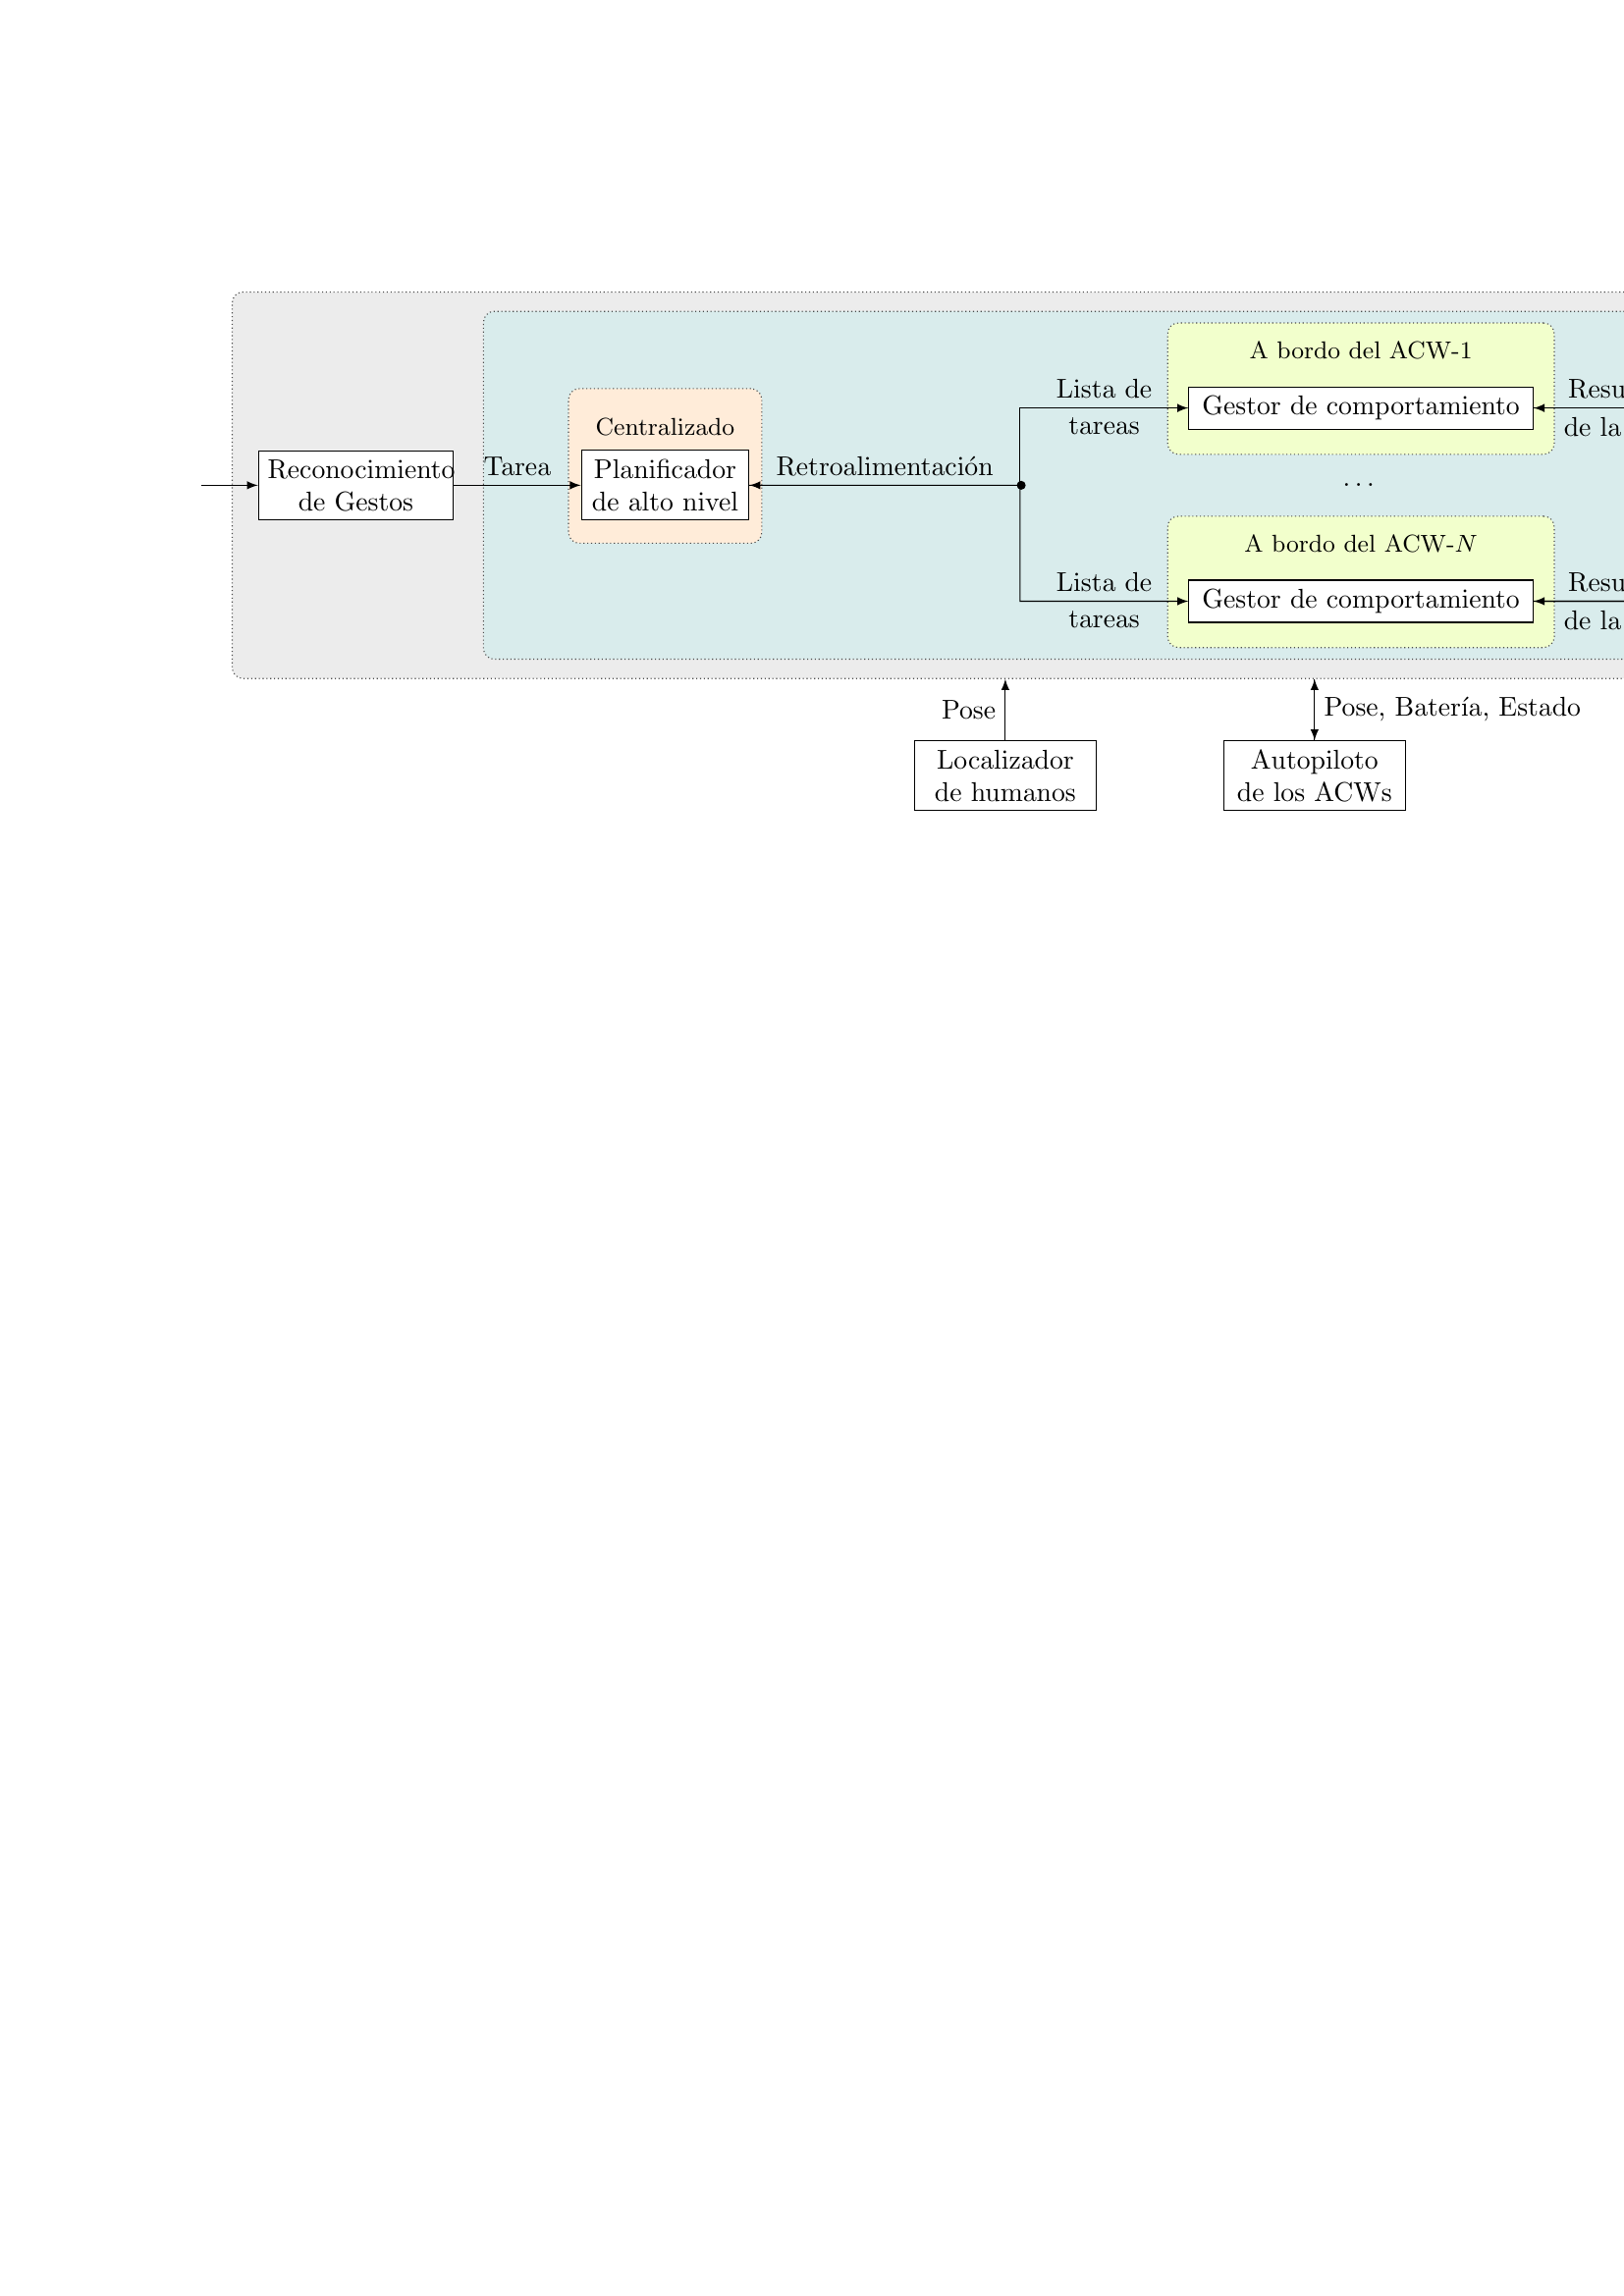
\begin{tikzpicture}
    		% WP7 block
    		\node (WP7-Box) at (10.4,0) [fill=gray!15,rounded corners, draw=black!70, densely dotted, minimum height=5cm, minimum width=24cm]{}; 

			% Task planner box
    		\node (TaskPlannerBox) at ($(WP7-Box)+(0.25,0)$) [fill=teal!15,rounded corners, draw=black!70, densely dotted, minimum height=4.5cm, minimum width=18cm]{};
    		
    		% Gesture Recognition
    		\node (GestureRecognition) at (0,0) [text centered, fill=white, draw, rectangle, minimum width=1.5cm, text width=6.5em]{Reconocimiento\\de Gestos};
    		
    		\draw[-latex] ($(GestureRecognition) - (2,0)$) -- (GestureRecognition);
 
    		% High-Level Planner
    		\node (HighLevelPlannerBox) at ($(GestureRecognition) + (4,0.25)$) [fill=orange!15,rounded corners, draw=black!70, densely dotted, minimum height=2cm, minimum width=2.5cm]{}; 
    		\node (HighLevelPlanner) at ($(HighLevelPlannerBox) + (0,-0.25)$) [text centered, fill=white, draw, rectangle, minimum width=1.5cm, text width=5.5em]{Planificador\\de alto nivel};
    		\node (Centralised) at ($(HighLevelPlanner) + (0,0.75)$) [text centered]{\small Centralizado};
    		
    		\draw[-latex] (GestureRecognition.east) -- node[above]{Tarea} (HighLevelPlanner);
    		
    		%%%%%%%%%%%%%%%%%%%
    		% UAV 1
    		\node (UAV1) at ($(HighLevelPlanner) + (9,1.25)$) [fill=lime!20,rounded corners, draw=black!70, densely dotted, minimum height=1.7cm, minimum width=5cm]{}; 
    		\node (AgentBehaviourManager1) at ($(UAV1) + (0,-0.25)$) [fill=white, draw, rectangle, text centered, text width=12em]{Gestor de comportamiento};
    		\node (UAV1-Text) at ($(AgentBehaviourManager1) + (0,0.75)$) [text centered]{\small A bordo del ACW-$1$};	

    		\draw[fill=black] ($ (HighLevelPlanner.east) + (3.465,0) $) arc(-180:180:0.05);
    		\draw[-latex] (HighLevelPlanner.east) -- ($ (HighLevelPlanner.east) + (3.5,0) $) -- ($ (HighLevelPlanner.east) + (3.5,1) $) -- node[above]{Lista de} node[below]{tareas} (AgentBehaviourManager1.west);
    		\draw[-latex] ($ (HighLevelPlanner.east) + (3.5,0) $) -- node[above]{Retroalimentación} (HighLevelPlanner.east);
    		
    		%%%%%%%%%%%%%%%%%%%
    		
    		% Dots
    		\node (Dots2) at ($(UAV1) + (0,-1.25)$) [text centered]{\dots};
    		
    		%%%%%%%%%%%%%%%%%%%
    		
    		% UAV N
    		\node (UAVN) at ($(HighLevelPlanner) + (9,-1.25)$) [fill=lime!20,rounded corners, draw=black!70, densely dotted, minimum height=1.7cm, minimum width=5cm]{}; 
    		\node (AgentBehaviourManagerN) at ($(UAVN) + (0,-0.25)$) [fill=white, draw, rectangle, text centered, text width=12em]{Gestor de comportamiento};
    		\node (UAVN-Text) at ($(AgentBehaviourManagerN) + (0,0.75)$) [text centered]{\small A bordo del ACW-$N$};	

    		\draw[-latex] (HighLevelPlanner.east) -- ($ (HighLevelPlanner.east) + (3.5,0) $) -- ($ (HighLevelPlanner.east) + (3.5,-1.5) $) -- node[above]{Lista de} node[below]{tareas} (AgentBehaviourManagerN.west);
    		
    		%%%%%%%%%%%%%%%%%%%
    		
    		% Lower-Level Controllers
    		\node (LowerLevelControllers) at ($(HighLevelPlanner) + (17,0)$) [text centered, fill=white, draw, rectangle, minimum width=1.5cm, text width=5.5em]{Controladores\\de nivel inferior};
    		
    		\draw[-latex] (LowerLevelControllers.east) -- ($(LowerLevelControllers) + (1.8,0)$);
    		
    		\draw[fill=black] ($ (LowerLevelControllers.west) + (-2.285,0) $) arc(-180:180:0.05);
    		\draw[-latex] (AgentBehaviourManager1.east) -- ($ (LowerLevelControllers.west) + (-2.25,1) $) -- ($ (LowerLevelControllers.west) + (-2.25,0) $) --  node[above]{Parámetros} node[below]{de la tarea}	(LowerLevelControllers.west);
    		\draw[-latex] (LowerLevelControllers.west) -- ($ (LowerLevelControllers.west) + (-2.25,0) $) -- ($ (LowerLevelControllers.west) + (-2.25,1) $) -- node[above]{Resultado} node[below]{de la tarea}	(AgentBehaviourManager1.east);
    		\draw[-latex] (AgentBehaviourManagerN.east) -- ($ (LowerLevelControllers.west) + (-2.25,-1.5) $) -- ($ (LowerLevelControllers.west) + (-2.25,0) $) -- (LowerLevelControllers.west);
    		\draw[-latex] (LowerLevelControllers.west) -- ($ (LowerLevelControllers.west) + (-2.25,0) $) -- ($ (LowerLevelControllers.west) + (-2.25,-1.5) $) -- node[above]{Resultado} node[below]{de la tarea} (AgentBehaviourManagerN.east);
    		
    		%%%%%%%%%%%%%%%%%%%%%
    		
    		\node (RealUAVs) at ($(WP7-Box.south) + (2,-1.25)$) [text centered, fill=white, draw, rectangle, minimum width=1.5cm, text width=6em]{Autopiloto\\de los ACWs};
    		\node (Humans) at ($(WP7-Box.south) + (-2,-1.25)$) [text centered, fill=white, draw, rectangle, minimum width=1.5cm, text width=6em]{Localizador\\de humanos};
    		
    		\draw[-latex] (RealUAVs.north) -- node[right]{Pose, Batería, Estado} ($(WP7-Box.south) + (2,0)$);
    		\draw[-latex] ($(WP7-Box.south) + (2,0)$) -- (RealUAVs.north);
    		\draw[-latex] (Humans.north) -- node[left]{Pose} ($(WP7-Box.south) + (-2,0)$);
		
	    \end{tikzpicture}}
	\caption{Arquitectura de software: bloques e interfaces. Diagrama de bloques desde la perspectiva del planificador de tareas cognitivas de alto nivel}
	\label{fig:NodeDiagram}
\end{figure}

%En el esquema de la arquitectura de software, aunque algunas comunicaciones son bidireccionales, se puede observar que existe un flujo principal de información. Empezando por la información que llega al módulo de \emph{Reconocimiento de Gestos}, ésta se propaga hasta la última capa, donde los \emph{Controladores de nivel inferior} utilizan la información ya procesada para dar órdenes al \glspl{ACW}. La tabla \ref{tab:interfaces} muestra el tipo de datos que cada uno de los módulos de la figura \ref{fig:NodeDiagram} recibe como entrada y el tipo de datos que cada uno de ellos envía como salida. Además, la tabla \ref{tab:shareddata} explica los detalles de los tipos de datos. 

% Description of the data interfaces for each software module
%\begin{table}[ht]
%    \centering
%    \caption{Descripción de las interfaces de datos para cada módulo de software}
%    \label{tab:interfaces}
%    \small
%    \begin{tabular}{|p{0.25\columnwidth}|p{0.25\columnwidth}|p{0.4\columnwidth}|}
%      \hline
%      \multicolumn{1}{|c}{\textbf{Nombre del módulo}} & \multicolumn{1}{|c|}{\textbf{Dato de entrada}} & \multicolumn{1}{c|}{\textbf{Dato de salida}}\\ \hline \hline
%      Reconocimiento de Gestos & Imágenes & \textbf{Tarea, definida por:} ID de la tarea, Tipo de la tarea, Distancia de monitorización, Número de monitorización, Lista de WPs, ID de la herramienta (algunos parámetros de tarea serán ignorados dependiendo del tipo de tarea) \\ \hline
%      
%     Planificador de alto nivel & Tarea, Retroalimentación (Resultado de la tarea, Batería suficiente, información del árbol de comportamiento (\gls{BT})), Pose del humano, Pose del \glspl{ACW}, Batería y Estado, y Baliza del agente & Lista de tareas añadiendo a cada una sus parámetros extra resultado de la planificación (Formación y/o Lista de IDs de los \glspl{ACW}) y Baliza del planificador\\\hline
%      
%      Gestor de comportamiento & Lista de tareas, Resultado del nivel inferior, Pose del humano, Pose del \glspl{ACW}, Batería y Estado & Parámetros necesarios para los controladores de bajo nivel (en función del tipo de tarea), Retroalimentación (resultado de la tarea, batería suficiente, información del BT) y Baliza del agente \\ \hline
%      
%      Controladores de nivel inferior & Parámetros (dependiendo del tipo de la tarea) & Resultado \\ \hline
%      
%      Localizador de humanos &  & Pose \\ \hline
%      
%      Autopiloto de los \glspl{ACW} & Órdenes de bajo nivel & Pose, Batería y Estado \\ \hline
%      
%    \end{tabular}
%\end{table}

% Description of data types
%\begin{table}[htb]
%    \centering
%    \caption{Descripción de los tipos de datos}
%    \label{tab:shareddata}
%    \small
%    \begin{tabular}{|p{0.2\columnwidth}|p{0.15\columnwidth}|p{0.55\columnwidth}|}
%      \hline
%      \multicolumn{1}{|c}{\textbf{Nombre del dato}} & \multicolumn{1}{|c|}{\textbf{Tipo del dato}} & \multicolumn{1}{c|}{\textbf{Comentario}} \\ \hline \hline
%      
%      ID de la tarea & Cadena & Identificador único de cada tarea \\ \hline
%      
%      Tipo de tarea & Entero & Indicador del tipo de tarea: m/M, i/I or d/D \\ \hline
%      
%      ID del humano & Cadena & Identificador único de cada trabajador humano. Se supone que la posición del objetivo humano y otra información necesaria es conocida y accesible a través de su ID. \\ \hline
%      
%      Distancia de monitorización & Flotante & Distancia desde la que los \glspl{ACW} vigilan al trabajador durante una tarea de monitorización de seguridad  \\ \hline
%      
%      Número de monitorización & Entero & Número de \glspl{ACW} que se requieren en la formación para una determinada tarea de monitorización de seguridad \\ \hline
%      
%      Lista de WPs & Lista de tuplas de $3$ flotantes ($x$, $y$, and $z$) & Lista de puntos a inspeccionar \\ \hline
%      
%      Lista de IDs de \glspl{ACW} & Lists de Cadenas & Lista de los identificadores únicos de los \glspl{ACW} que han sido seleccionados para una tarea que requiere múltiples \glspl{ACW} \\ \hline
%      
%      Formación & Entero & Indica cuál de los tipos de formaciones predefinidas debe utilizarse para la supervisión (por ejemplo, círculo, triángulo) \\ \hline
%      
%      ID de herramienta & Cadena & Identificador único de la herramienta a entregar \\ \hline
%      
%      Pode del \gls{ACW} & geometry\_msgs /PoseStamped & Posición y orientación del \gls{ACW}\\ \hline
%      
%      Batería del \gls{ACW} & sensors\_msgs /BatteryState & Porcentaje de batería del \gls{ACW} \\ \hline
%
%	    Resultado de la tarea & Cadena, Booleano & El primero es \gls{ID} único de la tarea y el segundo su resultado una vez terminada \\ \hline
%      
%      Batería suficiente & Booleano & Resultado de calcular si un \gls{ACW} tendrá suficiente batería para su tarea actual \\ \hline
%
%	    Información del \gls{BT} & Lista de Cadenas & Estado de cada nodo de \gls{BT} en su última ejecución (EN EJECUCIÓN, OCIOSO, ÉXITO o FALLO) \\ \hline
%      
%      Baliza del Agente & Cadena, Cadena & El primero es el ID único del \gls{ACW} mientras que el segundo define el tipo de \gls{ACW} (SafetyACW, InspectACW, o PhysicalACW). Se utiliza como latido y para detectar nuevos \glspl{ACW} en el Planificador de alto nivel \\ \hline
%
%	    Baliza del planificador & Tiempo & Mensaje de tipo ROS::Time que contiene el tiempo cuando la baliza fue mandada. Es usado para comprobar el estade de la conexión desde el lado del Agente. \\ \hline
%      
%      Resultado del nivel inferior & Booleano & Resultado de los controladores de nivel inferior una vez que han terminado después de ser llamados \\ \hline
%      
%    \end{tabular}
%\end{table}

El primer módulo comprueba constantemente las imágenes captadas por el \glspl{UAV} en busca de un gesto que indique una nueva tarea o la modificación de una tarea existente. Cuando esto ocurre, envía asíncronamente una tarea, que será recogida por el planificador centralizado. El \emph{Planificador de alto nivel}, cuando recibe esta información, procede a reevaluar el plan óptimo teniendo en cuenta la tarea recibida, la información que recibe de los \emph{Autopilotos de los \glspl{ACW}}, y la posición de los operarios, que es publicada periódicamente por el \emph{Localizador de humanos}. A bordo de cada \gls{ACW} hay un \emph{Gestor de comportamiento} que recoge la correspondiente lista de tareas proporcionada por el planificador centralizado, la información procedente del \emph{Localizador de humanos} y la del \emph{Autopiloto del \gls{ACW}} y se encarga de llamar a los \emph{Contoladores de nivel inferior} para llevar a cabo la ejecución del plan asignado. La información emitida por el \emph{Autopiloto del \gls{ACW}} se utiliza también para comprobar que todo funciona correctamente y para ejecutar los protocolos de seguridad en caso de que sean necesarios. Si esto ocurriera, se emitiría la correspondiente comunicación de vuelta al \emph{Planificador de alto nivel} para calcular un nuevo plan. Estos módulos también reciben el resultado de los \emph{Controladores de nivel inferior} después de llamar a cada uno de ellos, y lo publican de vuelta al \emph{Planificador de alto nivel} como retroalimentación. Además de estas comunicaciones, los módulos \emph{Planificador de alto nivel} y \emph{Gestor de comportamiento} de agente intercambian periódicamente balizas que sirven para detectar tanto la conexión de un nuevo \gls{ACW} como su desconexión en caso de fallo. 

\section{Módulo centalizado: Planificador de alto nivel}
\label{sec:Centralised module:TaskPlanner}
El \emph{Planificador de alto nivel} es un módulo centralizado que se ejecuta en una estación terrestre y constituye el principal módulo cognitivo de la arquitectura de software. Su objetivo es planificar la misión de forma óptima teniendo en cuenta el tiempo que se tarda en completar cada una, el tipo de cada \glspl{UAV}, la distancia que tendrá que recorrer cada uno, la batería que tienen disponible, la tarea que estaba ejecutando cada uno, la prioridad de cada tarea, la batería consumida por cada tarea, las recargas que serán necesarias, y cuándo es mejor realizar esas recargas.

El pseudocódigo general de este componente, desde el lanzamiento hasta la terminación, está representado en el código \ref{ps:GeneralPlanner}.

\begin{lstlisting}[caption={Pseudocódigo del bloque Planificador de alto nivel}, breaklines=true, label=ps:GeneralPlanner]
  1. Leer de un ros::param la dirección del archivo de configuración.
	2. Leer del archivo de configuración toda la información necesaria.
	3. Configurar las comunicaciones ROS (Publishers, Subscribers y ActionServers).
	4. Configurar la frecuencia de bucle.
	5. Bucle "while" principal". Mientras que ros::ok() y no misión terminada hacer:
		5.1. Comprobar el tiempo transcurrido de las balizas de los Agentes.
		5.2. Publicar una nueva baliza del Planificador.
		5.3. Comprobar si hay comunicaciones entrantes pendientes (ros::spinOnce).
		5.4. Dormir el tiempo restante para enviar la siguiente baliza.
	6. 6. Esperar a que todos los UAVs terminen y se desconecten. Mientras que haya algún agente conectado hacer:
		6.1. Comprobar el tiempo transcurrido de las balizas de los agentes.
		6.2. Comprobar si hay comunicaciones entrantes pendientes (ros::spinOnce).
		6.3. Dormir un rato.
\end{lstlisting}

%Dado que el entorno en el que operan los \glspl{UAV} es dinámico, este módulo se ha programado de forma que pueda reaccionar ante los imprevistos y recalcular el plan óptimo. Como se puede deducir del código \ref{ps:GeneralPlanner}, todo funciona a través de funciones de respuesta. Cada vez que llega una comunicación desde otro nodo de \acrshort{ROS}, se activa una respuesta en este nodo. En ella se analiza la información contenida en el mensaje y se decide si es necesaria una replanificación o no. Las situaciones en las que se ha considerado necesaria una replanificación se enumeran en la sección \ref{sec:TaskReplanningSituations}. Las comunicaciones resumidas en las tablas \ref{tab:interfaces} y \ref{tab:shareddata} y en la figura \ref{fig:NodeDiagram} son suficientes para detectar estos imprevistos y poder responder a ellos de la mejor manera posible.

%\begin{lstlisting}[caption={Pseudocódico de la respuesta a nueva tarea}, breaklines=true, label=ps:IncomingTask]
%	1. Si la tarea ya existe:
%		1.1. Si el tipo de la nueva tarea es el mismo que el de la antigua:
%			1.1.1. Actualizar los parámetros, realizar una planificación de la tarea y return.
%		1.2. Si no: Avisar a los operadores de que se va a eliminar una tarea pendiente y eliminar la tarea antigua.
%	2. Leer el tipo de tarea y los parámetros que le corresponden.
%	3. Añadir la nueva tarea a la lista de tareas pendientes.
%	4. Realizar una planificación de tareas.
%\end{lstlisting}

%Existe una respuesta que se ejecuta cuando el nodo \emph{Reconocimiento de gestos} envía una tarea, que en caso de que la tarea dada sea correcta, siempre acaba llamando a la función encargada de calcular el plan óptimo (ver código \ref{ps: IncomingTask}); la función respuesta a la señal de fin de misión, cuya única acción es cambiar el valor de una variable para que el nodo salga del bucle while principal; y por último la función respuesta a la baliza del agente, que se ejecuta cada vez que se recibe una baliza \gls{UAV} y cuyo pseudocódigo está en Code \ref{ps:AgentBeaconCallback}.

%\begin{lstlisting}[caption={Pseudocódigo de la función respuesta a la baliza del agente}, breaklines=true, label=ps:AgentBeaconCallback]
%	1. Leer la información contenida en la baliza.
%	2. Si se trata de una conexión de un nuevo UAV:
%		2.1. Registrarlo en la base de datos.
%		2.2. Ejecutar una planificación de tareas.
%	3. Si es el latido de un UAV ya conocido:
%		3.1. Reiniciar su temporizador.
%\end{lstlisting}

%La acción que realiza la función respuesta de la baliza del agente varía en función de si es la baliza de un nuevo \gls{UAV} o el latido de un \gls{UAV} conocido. Para cada agente habrá un objeto en la base de datos que contendrá otra serie de funciones de respuesta que se encargarán de recibir los mensajes procedentes del \glspl{ACW} y responder en consecuencia.

%\begin{lstlisting}[caption={Funcion de respuesta que se ejecuta cuando un \emph{Gestor de comportamiento} de agente envía información sobre la batería}, breaklines=true, label=ps:batteryEnoughCB]
%	1. Actualizar el valor de la bandera interna asociada a la batería.
%	2. Realizar una planificación de tareas.
%\end{lstlisting}

%El bloque \emph{Gestor de comportamiento} sólo envía mensajes de comunicación indicando el estado de la batería cuando se debe a un evento no planificado. Este evento puede ser un agotamiento temprano de la batería o una recarga más rápida de lo esperado. En ambos casos, la función de respuesta, cuyo pseudocódigo es el código \ref{ps:batteryEnoughCB}, actualiza el valor de una variable interna utilizada durante la planificación, y recalcula el plan óptimo.

%La otra comunicación posible procedente de un nodo de tipo \emph{Gestor de comportamiento} con capacidad para desencadenar una reacción en el planificador se debe a la finalización de una tarea. Cuando una tarea termina con éxito, simplemente se elimina de la lista de tareas pendientes. En este caso, el bloque \emph{Gestor de comportamiento} también elimina la tarea de su cola, que es el único caso en el que lo hace. Además, este momento se aprovecha para reevaluar el plan óptimo. Se espera que la misión siga estando dentro del plan óptimo, por lo que en ese caso el resultado de la planificación debería ser el mismo que el del plan que ya se estaba ejecutando. Si, en cambio, las condiciones han cambiado desde la última planificación y ahora existe un plan mejor, es en este momento cuando se actualiza el plan. Si la tarea termina con un fallo, la acción de la función de respuesta dependerá de las causas del fallo (tener en cuenta que la interrupción de una tarea dará lugar a un fallo). Si la interrupción se debe a la batería, puede ser planificada, en cuyo caso no se requiere ninguna acción, o puede ser inesperada, en cuyo caso las acciones correspondientes son tomadas por la función de respuesta de la batería. Una vez comprobado que la tarea no ha terminado por culpa de la batería, se comprueba si la tarea estaba al principio de la cola. Si es así, efectivamente se ha producido un fallo, por lo que se avisa a los operadores, se elimina la tarea de la lista y se ejecuta una nueva planificación. En caso contrario, la tarea en cuestión se habría desplazado del principio de la cola debido a un cambio de planes y, por tanto, tampoco habría que realizar ninguna acción. El pseudocódigo correspondiente a lo que se acaba de explicar se encuentra en el Código \ref{ps:taskResultCB}.

%\begin{lstlisting}[caption={Función de respuesta que se ejecuta cuando un \emph{Gestor de comportamiento} comunica el resultado de una tarea}, breaklines=true, label=ps:taskResultCB]
%	1. Leer la información contenida en el resultado de la tarea.
%	2. Si el resultado de la tarea es ÉXITO:
%		2.1. Eliminarla de la lista de tareas pendientes.
%		2.2. Realizar una planificación de la tarea.
%	3. En caso contrario, si el resultado de la tarea es FALLO:
%		3.1. Si la tarea se ha detenido por no tener batería suficiente:
%			3.1.1. Return.
%		3.2. En caso contrario, si la tarea está al frente de la cola de tareas de ese ACW:
%			3.2.1. Notificar a los operadores que una tarea ha fallado y va a ser eliminada.
%			3.2.2. Eliminar la tarea de la lista de tareas pendientes.
%			3.2.3. Realizar una planificación de tareas.
%		3.3. Si no:
%			3.3.1. Return.
%\end{lstlisting}

%Las otras dos comunicaciones que recibe el \emph{Planificador de alto nivel} de los \glspl{ACW} son las lecturas de los sensores correspondientes a la posición de los \glspl{UAV} y el porcentaje de batería. En ambos casos la única acción del callback correspondiente es actualizar la información con los nuevos valores.

%La última función que queda por explicar de las que potencialmente pueden solicitar una replanificación de la misión es la encargada de comprobar el tiempo límite de las balizas de los agentes. Como se muestra en el Código \ref{ps:GeneralPlanner}, esta función no es una función de respuesta como las anteriores, sino que se ejecuta periódicamente en el bucle while principal. Su funcionamiento se muestra en el Código \ref{ps:checkBeaconsTimeout}. Básicamente, para cada agente conectado, comprueba que no ha transcurrido el tiempo máxmio desde que se recibió su última baliza. Si ha transcurrido el tiempo máximo, ese \gls{ACW} se considera desconectado y se elimina de la base de datos del nodo centralizado. Si, tras comprobar todos los agentes, el número de \glspl{UAV} conectados ha disminuido, es decir, si alguno de los \glspl{UAV} previamente conectados se ha desconectado, se ejecuta una replanificación de la misión.

% Pseudocódigo de checkBeaconsTimeout
%\begin{lstlisting}[caption={Función que comprueba el tiempo límite de las balizas de los agentes}, breaklines=true, label=ps:checkBeaconsTimeout]
%	1. Por cada agente conectado:
%		1.1. Si el tiempo transcurrido desde la última baliza es mayor que el tiempo máximo:
%			1.1.1. Añadir el ID de ese agente a la lista de agentes desconectados.
%	2. Mientras la lista de agentes desconectados no esté vacía:
%		2.1. Tomar el primer ID de la lista.
%		2.2. Borrar de los datos del bloque toda la información relacionada con ese ID.
%	3. Si algún agente se ha desconectado:
%		3.1. Ejecutar una planificación de tareas.
%\end{lstlisting}

%El pseudocódigo que se ejecuta cuando es necesario realizar una nueva planificación de tareas se resume en el Código \ref{ps:performTaskAllocation}. Es importante recordar que algunas tareas tienen mayor prioridad que otras, y esto depende únicamente del tipo de tarea. Para simplificar el proceso, se ha decidido asignar las tareas por orden de llegada, asumiendo que entre dos tareas del mismo tipo, tendrá prioridad la que haya llegado primero. Cuando se recibe una nueva tarea, se almacena tanto en un \emph{std::map} que contiene todas las tareas pendientes para facilitar el acceso a la información, como en un \emph{std::vector} con los tipos de tareas, donde se mantiene el orden de llegada. Lo que permite esta simplificación es asignar las tareas de una en una. Al disponer de una lista priorizada de tareas y asumir que ninguna tarea puede ser asignada antes que otra de mayor prioridad, el problema de planificación de la misión se reduce a calcular el coste de cada tarea individualmente para cada \gls{UAV} con capacidad de ejecutarla y asignarla a la de menor coste. En el caso de las tareas de monitorización, la selección del número necesario de agentes se basa estrictamente en el coste. Se seleccionan los \emph{N} agentes a los que menos cueste ejecutar la tarea. Esto es un poco más complejo para las tareas de tipo inspeccionar, donde el número de agentes a seleccionar es un parámetro a definir por el propio planificador. Este valor se establece primero en función del número de puntos a inspeccionar. Hasta tres puntos, se selecciona un único agente; hasta seis puntos, se seleccionan dos; y a partir de siete puntos, se seleccionan tres agentes, siendo éste el número máximo impuesto por el controlador de bajo nivel. Además, tal y como trabaja el controlador de bajo nivel encargado de esta tarea, se requiere que todos los \glspl{ACW} seleccionados para esta tarea comiencen a ejecutarla simultáneamente, por lo que se realiza una segunda aproximación de este número en función del número de \glspl{UAV} ociosos. Así, si se les asigna como primera tarea, comenzarán a ejecutarla simultáneamente. Académicamente, esta simplificación parece desviarse de la solución óptima, pero hay que recordar que este trabajo forma parte de una arquitectura de software que funcionará en situaciones reales. En dichas situaciones, no se espera que haya un gran número de \glspl{UAV} conectados simultáneamente, ni una larga lista de tareas pendientes. En estos escenarios simplificados, esta suposición tiene sentido sin desviarse demasiado de la solución óptima. Finalmente, el número de agentes a seleccionar será el menor de los dos anteriores, siendo igual a uno cuando no haya ningún \gls{UAV} ocioso y cero en caso de que no haya ningún \gls{ACW} con suficiente batería. En este último caso, la tarea se asignaría tras la recarga. Una vez definido el número de agentes a seleccionar, se seleccionan los agentes que tienen menor coste para ejecutar la tarea de entre los que cumplen las condiciones descritas. Una vez seleccionados los \gls{ACW} que van a realizar la tarea, sólo queda distribuir entre ellos los \glspl{WP} a inspeccionar. Aunque el algoritmo encargado de realizar la distribución óptima se encuentra en el controlador de bajo nivel de esta tarea, al no disponer aún del resto de módulos que componen la arquitectura software, ha sido necesario programar un algoritmo de distribución para poder realizar los experimentos. En la sección \ref{sec:faking} se darán más detalles al respecto.

%El coste de cada \gls{UAV} se calcula como la suma ponderada de tres tipos de costes diferentes. Un primer coste evalúa el tipo de \gls{ACW} y penaliza la asignación de tareas a aquellos \glspl{UAV} diseñados para otro tipo. Penaliza especialmente la asignación de tareas de menor prioridad a agentes diseñados para realizar tareas de mayor prioridad. El segundo coste evalúa la distancia total que tendrá que recorrer el \gls{UAV} desde donde se encuentra al principio de la tarea hasta donde debería estar al final de la misma. Este coste es una aproximación al consumo de batería previsto, aunque no tiene en cuenta los tiempos intermedios de desplazamiento y de vuelo estático durante la tarea. El último coste penaliza la interrupción de la tarea que se estaba ejecutando según el plan anterior y premia la asignación de la misma tarea. Este coste pretende que se asigne preferentemente una tarea a un \gls{UAV} inactivo, a un \gls{UAV} que esté ejecutando una tarea de menor prioridad, o incluso a un \gls{UAV} de distinto tipo, en lugar de interrumpir innecesariamente una tarea sólo porque ese \gls{UAV} tenga que recorrer una distancia menor, por ejemplo.

%\begin{lstlisting}[caption={Pseudocódigo de la función que hace la planifiación de tareas}, breaklines=true, label=ps:performTaskAllocation]
%	1. Si hay algún agente conectado:
%		1.1. Por cada agente conectado:
%			1.1.1. Hacer una copia de la cola de tareas actual.
%			1.1.2. Vaciar la cola de tareas.
%		1.2. Para cada tarea de entrega de herramientas:
%			1.2.1. Calcular el coste de la tarea para cada PhysicalACW que tenga suficiente batería.
%			1.2.2. Asignar la tarea al agente al que le cueste menos la tarea (de los que tienen suficiente batería).
%			1.2.3. Añadir la tarea a la cola de tareas de ese agente.
%		1.3. Para cada tarea de inspección:
%			1.3.1. Extraer de los parámetros de la tarea la lista de WP a inspeccionar.
%			1.3.2. Para cada ACW (de cualquier tipo) que tenga suficiente batería:
%				1.3.2.1. Calcular el coste de la tarea para ese ACW. 
%				1.3.2.2. Comprobar si ese ACW sigue estando inactivo.
%			1.3.3. Calcular el número de agentes a seleccionar para la tarea en función del número de WP y del número de agentes ociosos.
%			1.3.4. Si ningún agente tiene suficiente batería, continuar.
%			1.3.5. Si el número de agentes a seleccionar es igual a cero, se asigna la tarea al agente que menos cuesta.
%			1.3.6. En caso contrario, seleccione el número calculado de agentes para los que la tarea cuesta menos.
%			1.3.7. Dividir el WP a inspeccionar entre los agentes seleccionados.
%			1.3.8. Para cada agente seleccionado:
%				1.3.8.1. Establecer el resto de parámetros de la tarea (Lista de IDs de ACWs seleccionados y lista de WP divididos).
%				1.3.8.2. Añadir la tarea a la cola de tareas del agente.
%		1.4. Para cada tarea de Monitorización:
%			1.4.1. Calcular el coste de la tarea para cada ACW (de cualquier tipo) que tenga suficiente batería.
%			1.4.2. Si el número de ACW necesarios para la tarea es cero:
%				1.4.2.1. Advertir a los operadores que este parámetro no puede ser cero.
%				1.4.2.2. Eliminar la tarea de las tareas pendientes.
%			1.4.3. Si no, seleccionar el número de agentes solicitados para los que la tarea cuesta menos.
%			1.4.4. Establecer el parámetro de la tarea restante (Lista de IDs de ACWs seleccionados)
%			1.4.4. Añadir la tarea a la cola de tareas de cada agente seleccionado.
%		1.5. Por cada ACW conectado, enviar la nueva cola de tareas a su Gestor de comportamiento.
%	2. Si no:
%		2.1. Avisar a los operadores de que no hay ningún agente conectado.
%\end{lstlisting}

%Una vez finalizado el cálculo del plan de la misión, las nuevas colas de tareas se envían a los módulos distribuidos correspondientes. Cada \emph{Gestor de comportamiento} reaccionará a esta comunicación y se encargará de ejecutar el nuevo plan asignado. Mientras tanto, el bloque \emph{Planificador de alto nivel} vuelve al bucle while principal para seguir esperando hasta que se produzca de nuevo un evento que desencadene una replanificación.

\section{Módulo distribuido: Gestor de comportamiento}
\label{sec:Distributed module: behaviour manager}
Este componente se encarga de ejecutar el plan asignado por el \emph{Planificador de alto nivel}, comprobando en todo momento la seguridad de los \glspl{UAV}, detectando los imprevistos y comunicándolos al nodo centralizado para que realice un cambio de planes en caso necesario. El \emph{Gestor de comportamiento} se comunicará con los controladores de bajo nivel, cediendo el control cuando sea necesario para completar el plan asignado.

La estructura general de este módulo es bastante similar a la del módulo central. El pseudocódigo se resume en el Código \ref{ps:GeneralAgent}. Tras la inicialización, el \emph{Gestor de comportamiento} prepara la información necesaria para comenzar su funcionamiento, configura las comunicaciones necesarias, declara e inicializa el árbol de comportamiento y, una vez que el \gls{UAV} ha terminado de inicializarse, comienza a enviar balizas al nodo central para notificar que se incorpora a la misión. Una vez que el código termina de inicializarse y llega al bucle while principal, la actividad del \emph{Gestor de comportamiento} se concentra en la ejecución de funciones en respuesta a los mensajes entrantes, como las de el \emph{Planificador de alto nivel}, y en la ejecución del árbol de comportamiento, que dirige y supervisa el movimiento del \gls{UAV}.

\begin{lstlisting}[caption={Pseudocódigo del bloque \emph{Gestor de comportamiento}}, breaklines=true, label=ps:GeneralAgent]
	1. Leer de un ros::param el contenido de la baliza (ID y tipo de ACW).
	2. Leer de un ros::param la dirección del archivo de configuración.
	3. Leer del archivo de configuración toda la información necesaria.
	4. Configurar las comunicaciones de ROS (Publishers, Subscribers y ActionServers).
	5. Configurar la frecuencia del bucle.
	6. Declarar el árbol de comportamiento.
	7. Inicializar cada nodo del BT.
	8. Iniciar los registradores del BT para facilitar la depuración y el seguimiento del rendimiento del nodo.
	9. Esperar a que el ACW se inicialice completamente.
	10. Bucle "while" principal. Mientras ros::ok() y el estado de BT es EN EJECUCIÓN:
		10.1. Si no se ha producido un timeout de las balizas del Planificador:
			10.1.1. Publicar una nueva baliza del Agente.
		10.2. Compruebar si la batería es suficiente para la tarea actual.
		10.3. Compruebar si hay comunicaciones entrantes pendientes (ros::spinOnce).
		10.4. Dormir el tiempo restante para enviar la siguiente baliza.
\end{lstlisting}

Los \glspl{BT} son quienes gobiernan a los \glspl{ACW} para realizar cada una de las tareas asignadas. Cada \gls{BT} monitoriza el estado de la batería y de las tareas de su \gls{ACW} y reacciona ante cualquier posible fallo o imprevisto, solicitando una nueva replanificación al \emph{Planificador de alto nivel} en caso de necesidad. Un \gls{BT} puede definirse como una máquina finita de estados (\gls{FSM}) mejorada. Son un mecanismo más avanzado para implementar comportamientos, especialmente por sus ventajas en términos de escalabilidad, modularidad, legibilidad y reutilización, facilitando la creación de comportamientos más complejos con menos esfuerzo.

%A pesar de esto, el proceso de diseño de una \gls{FSM} es bastante diferente al proceso de diseño de un \gls{BT}. Diseñar \glspl{BT} sin haberlo hecho antes no es una tarea trivial. Además, habrá más de una implementación válida para conseguir el mismo comportamiento, lo que hace más complicado diseñar este tipo de soluciones cuando aún no se tiene la suficiente intuición para saber cuál es la mejor. Aprovechando que el uso de \glspl{BT} está muy extendido en la industria de los videojuegos, se recopiló y estudió información sobre ellos para intentar desarrollar el conocimiento y la intuición suficientes para diseñar desde cero un \gls{BT} que cumpla con las necesidades de la misión. Para ello, fueron muy útiles los ejemplos previos encontrados en \cite{BT-CPP-doc, colledanchise2018behavior, BT-AI}.

%Antes de proceder a la explicación del \gls{BT} diseñado, se comentarán brevemente los tipos de nodos que se pueden encontrar en la biblioteca C++ seleccionada (ver Figura~\ref{fig:BTnodes}) y el funcionamiento de cada uno de ellos.

%% Tipos de nodos de BT
%\begin{figure}[htbp]
%    \centering
%    \subfloat[]{%Fallback
%		\label{subfig:Fallback}
%        \begin{tikzpicture}
%			\node (MainTree) at (0,0) [text centered, fill=white, draw, rectangle, minimum width=0.5cm, text width=0.5em]{\textbf{?}};
%		\end{tikzpicture}}
%    \hfill
%    \subfloat[]{%Sequence
%		\label{subfig:Sequence}
%        \begin{tikzpicture}
%			\node (MainTree) at (0,0) [text centered, fill=white, draw, rectangle, minimum width=1.5cm, text width=1.5em]{$\longrightarrow$};
%		\end{tikzpicture}}
%	\hfill
%    \subfloat[]{%Reactive
%		\label{subfig:Reactive}
%        \begin{tikzpicture}
%			\node (MainTree) at (0,0) [text centered, fill=magenta!5, draw=magenta, rectangle, minimum width=2cm, minimum height=0.75cm, text width=2em]{};
%		\end{tikzpicture}}
%    \hfill
%    \subfloat[]{%Common
%		\label{subfig:Common}
%        \begin{tikzpicture}
%			\node (MainTree) at (0,0) [text centered, fill=white, draw, rectangle, minimum width=2cm, minimum height=0.75cm, text width=2em]{};
%		\end{tikzpicture}}
%    \hfill
%    \subfloat[]{%Decorator
%		\label{subfig:Decorator}
%        \begin{tikzpicture}
%			\node (MainTree) at (0,0) [text centered, fill=orange!5, draw=orange, rectangle, minimum width=2cm, minimum height=0.75cm, text width=2em]{};
%		\end{tikzpicture}}
%    \hfill
%    \subfloat[]{%Action
%		\label{subfig:Action}
%		\begin{tikzpicture}
%			\node (MainTree) at (0,0) [text centered, fill=blue!5, draw=blue, rectangle, minimum width=2cm, minimum height=0.75cm, text width=2em]{};
%		\end{tikzpicture}}
%		\hfill
%    \subfloat[]{%Condition
%		\label{subfig:Condition}
%        \begin{tikzpicture}
%			\node (MainTree) at (0,0) [text centered, fill=blue!5, draw=blue, ellipse, minimum width=2cm, minimum height=0.75cm, text width=2em]{};
%		\end{tikzpicture}}
%    \caption{Diferentes tipos de nodos que pueden estar presentes en un \gls{BT}}
%    \label{fig:BTnodes}
%\end{figure}

%Los Árboles de Comportamiento están formados por nodos de \emph{Control}, nodos \emph{Decoradores} y nodos \emph{Hoja}. Los nodos de \emph{Control} pueden ser nodos de \emph{Alternativa}, representados con un signo de interrogación (ver subfigura \ref{subfig:Fallback}), que intentan tener éxito llamando uno a uno a cada uno de sus hijos; o nodos \emph{Secuancia}, representados con una flecha (ver subfigura \ref{subfig:Sequence}), que llaman a sus hijos en orden si el anterior ha tenido éxito. Por un lado, los nodos \emph{Alternativa} devuelven \emph{ÉXITO} si uno de sus hijos lo hace, \emph{FALLO} si ninguno tiene éxito, y \emph{EN EJECUCIÓN} si uno de sus hijos devuelve \emph{EN EJECUCIÓN}. Por otro lado, los nodos \emph{Secuencia} devuelven \emph{ÉXITO} cuando todos los hijos han sido llamados en orden y han devuelto \emph{ÉXITO}. Si alguno de ellos devuelve \emph{FALLO}, la secuencia se rompe y el nodo \emph{Secuencia} devuelve \emph{FALLO} también. Cuando un hijo devuelve \emph{EN EJECUCIÓN}, el nodo \emph{Secuencia} también lo hace. Los nodos de \emph{Control} se representan con un recuadro rectangular negro cuando son comunes (ver subfigura \ref{subfig:Common}), pero también pueden ser nodos de control \emph{Reactivos}, representados por un recuadro magenta (ver subfigura \ref{subfig:Reactive}), lo que significa que sus hijos ya llamados serán llamados de nuevo en la siguiente iteración. Esto es muy útil para generar comportamientos en los que una acción se reintenta constantemente, o en los que es necesario comprobar que se siguen cumpliendo las condiciones requeridas. Un nodo \emph{Hijo} puede ser otro nodo de \emph{Control}, un nodo \emph{Decorador}, un nodo \emph{Hoja} o un subárbol completo. Un nodo \emph{Decorador}, representado en un recuadro naranja (véase la subfigura \ref{subfig:Decorator}), sólo puede tener un hijo (de cualquier tipo) y su función es programable (por ejemplo, modificar el resultado de su hijo o reintentar llamar a su hijo un número de veces). Los nodos \emph{Hoja}, representados en azul, pueden ser nodos de \emph{Condición}, representados en una caja azul de forma elíptica (véase la subfigura \ref{fig:Condition}), que comprueban una condición y devuelven \emph{ÉXITO} o \emph{FALLO}; o nodos de \emph{Acción}, representados en una caja rectangular azul (véase la subfigura \ref{subfig:Action}), que ejecutan un código que lleva más tiempo y, por tanto, estos nodos también podrían devolver \emph{EN EJECUCIÓN}.

\subsection{Árbol principal}
\label{sec:MainTree}
%En general, el diseño tanto del \gls{BT} como del \emph{Gestor de comportamiento} se ha realizado con el objetivo de concentrar la menor inteligencia posible que garantice el éxito de la misión y la seguridad de los \glspl{UAV} y de los trabajadores. Por ello, la única tarea de las funciones de respuesta que se ejecutan cuando llegan diferentes mensajes es actualizar el valor de las variables internas correspondientes. 

%Sin embargo, no toda la inteligencia y la toma de decisiones pueden situarse en el nodo de la estación de tierra. Tiene que haber cierta capacidad de decisión a bordo de los \glspl{UAV} en caso de que se pierda la conexión con el nodo central. Por eso hay un protocolo predefinido para actuar cuando esto ocurre o cuando la batería se agota antes de lo previsto. Estos dos factores se comprueban periódicamente en el bucle while principal (véase el código \ref{ps:GeneralAgent}). En el caso de la batería, si la función encargada determina que no hay suficiente batería para completar la tarea actual, lo que ocurre es que se vacía la cola de tareas y se actualiza el valor de la bandera interna asociado a la batería. Además, el evento se comunica al planificador de tareas en caso de que la conexión siga viva para generar un nuevo plan. Del mismo modo, si se detecta una pérdida de conexión, se vacía la cola de tareas y se actualiza la bandera correspondiente. En este caso, el bloque \emph{Planificador de alto nivel} ejecutará una replanificación cuando también detecte la pérdida de conexión.

%El \gls{BT} está diseñado de forma que, cuando la cola de tareas se vacía y se actualizan las banderas respectivas, el \gls{UAV} correspondiente se dirige a la estación de carga de batería, que es el protocolo de emergencia establecido. Para activar el protocolo en caso de emergencia solo hay que vaciar la cola de tareas y comunicarlo al bloque central. En el caso de que la conexión entre los dos nodos siga activa pero no haya suficiente batería, el objetivo del plan de contingencia es eliminar los riesgos para el \gls{UAV} mientras el \emph{Planificador de alto nivel} genera nuevas instrucciones. Además, es probable que el nuevo plan implique la recarga de la batería como primer paso. Por otro lado, el peligro de la pérdida de la conexión es que si el \gls{ACW} desconectado continúa con el último plan asignado, podrían producirse colisiones. El protocolo de emergencia garantiza que el \gls{UAV} desconectado no interfiera con los nuevos planes. Además, el tiempo hasta el restablecimiento de la conexión se aprovecha para recargar la batería, lo que es positivo para la misión.

%Los \glspl{BT} operan de forma recursiva. Todos los nodos, independientemente de su tipo, tienen una función que ejecuta su contenido, la función \emph{tick}. Cuando se hace \emph{tick} al nodo raíz desde el bucle while principal, este propaga el \emph{tick} entre sus hijos siguiendo las reglas de funcionamiento descritas en la Sección \ref{sec:Distributed module: behaviour manager} hasta que finalmente un nodo \emph{Hoja} devuelve una de las tres respuestas posibles (\emph{ÉXITO}, \emph{EN EJECUCIÓN} o \emph{FALLO}), que se propagará de vuelta, para obtener un resultado final que devolverá el nodo raíz. Como la función de este \gls{BT} es controlar durante toda la misión el movimiento de un \gls{UAV}, se ha definido un nodo \emph{Decorador} que siempre devuelve \emph{EN EJECUCIÓN} independientemente del resultado de su nodo hijo. El \gls{BT} implementado como solución al problema descrito se divide a su vez en varios \glspl{BT}, aprovechando la modularidad que ofrece este enfoque. El árbol principal se representa en la Figura \ref{fig:MainTree}, siendo el nodo denominado como \emph{Main Tree} la raíz del árbol completo.

\begin{figure}[ht]
	\begin{center}
		\scalebox{0.9}{
			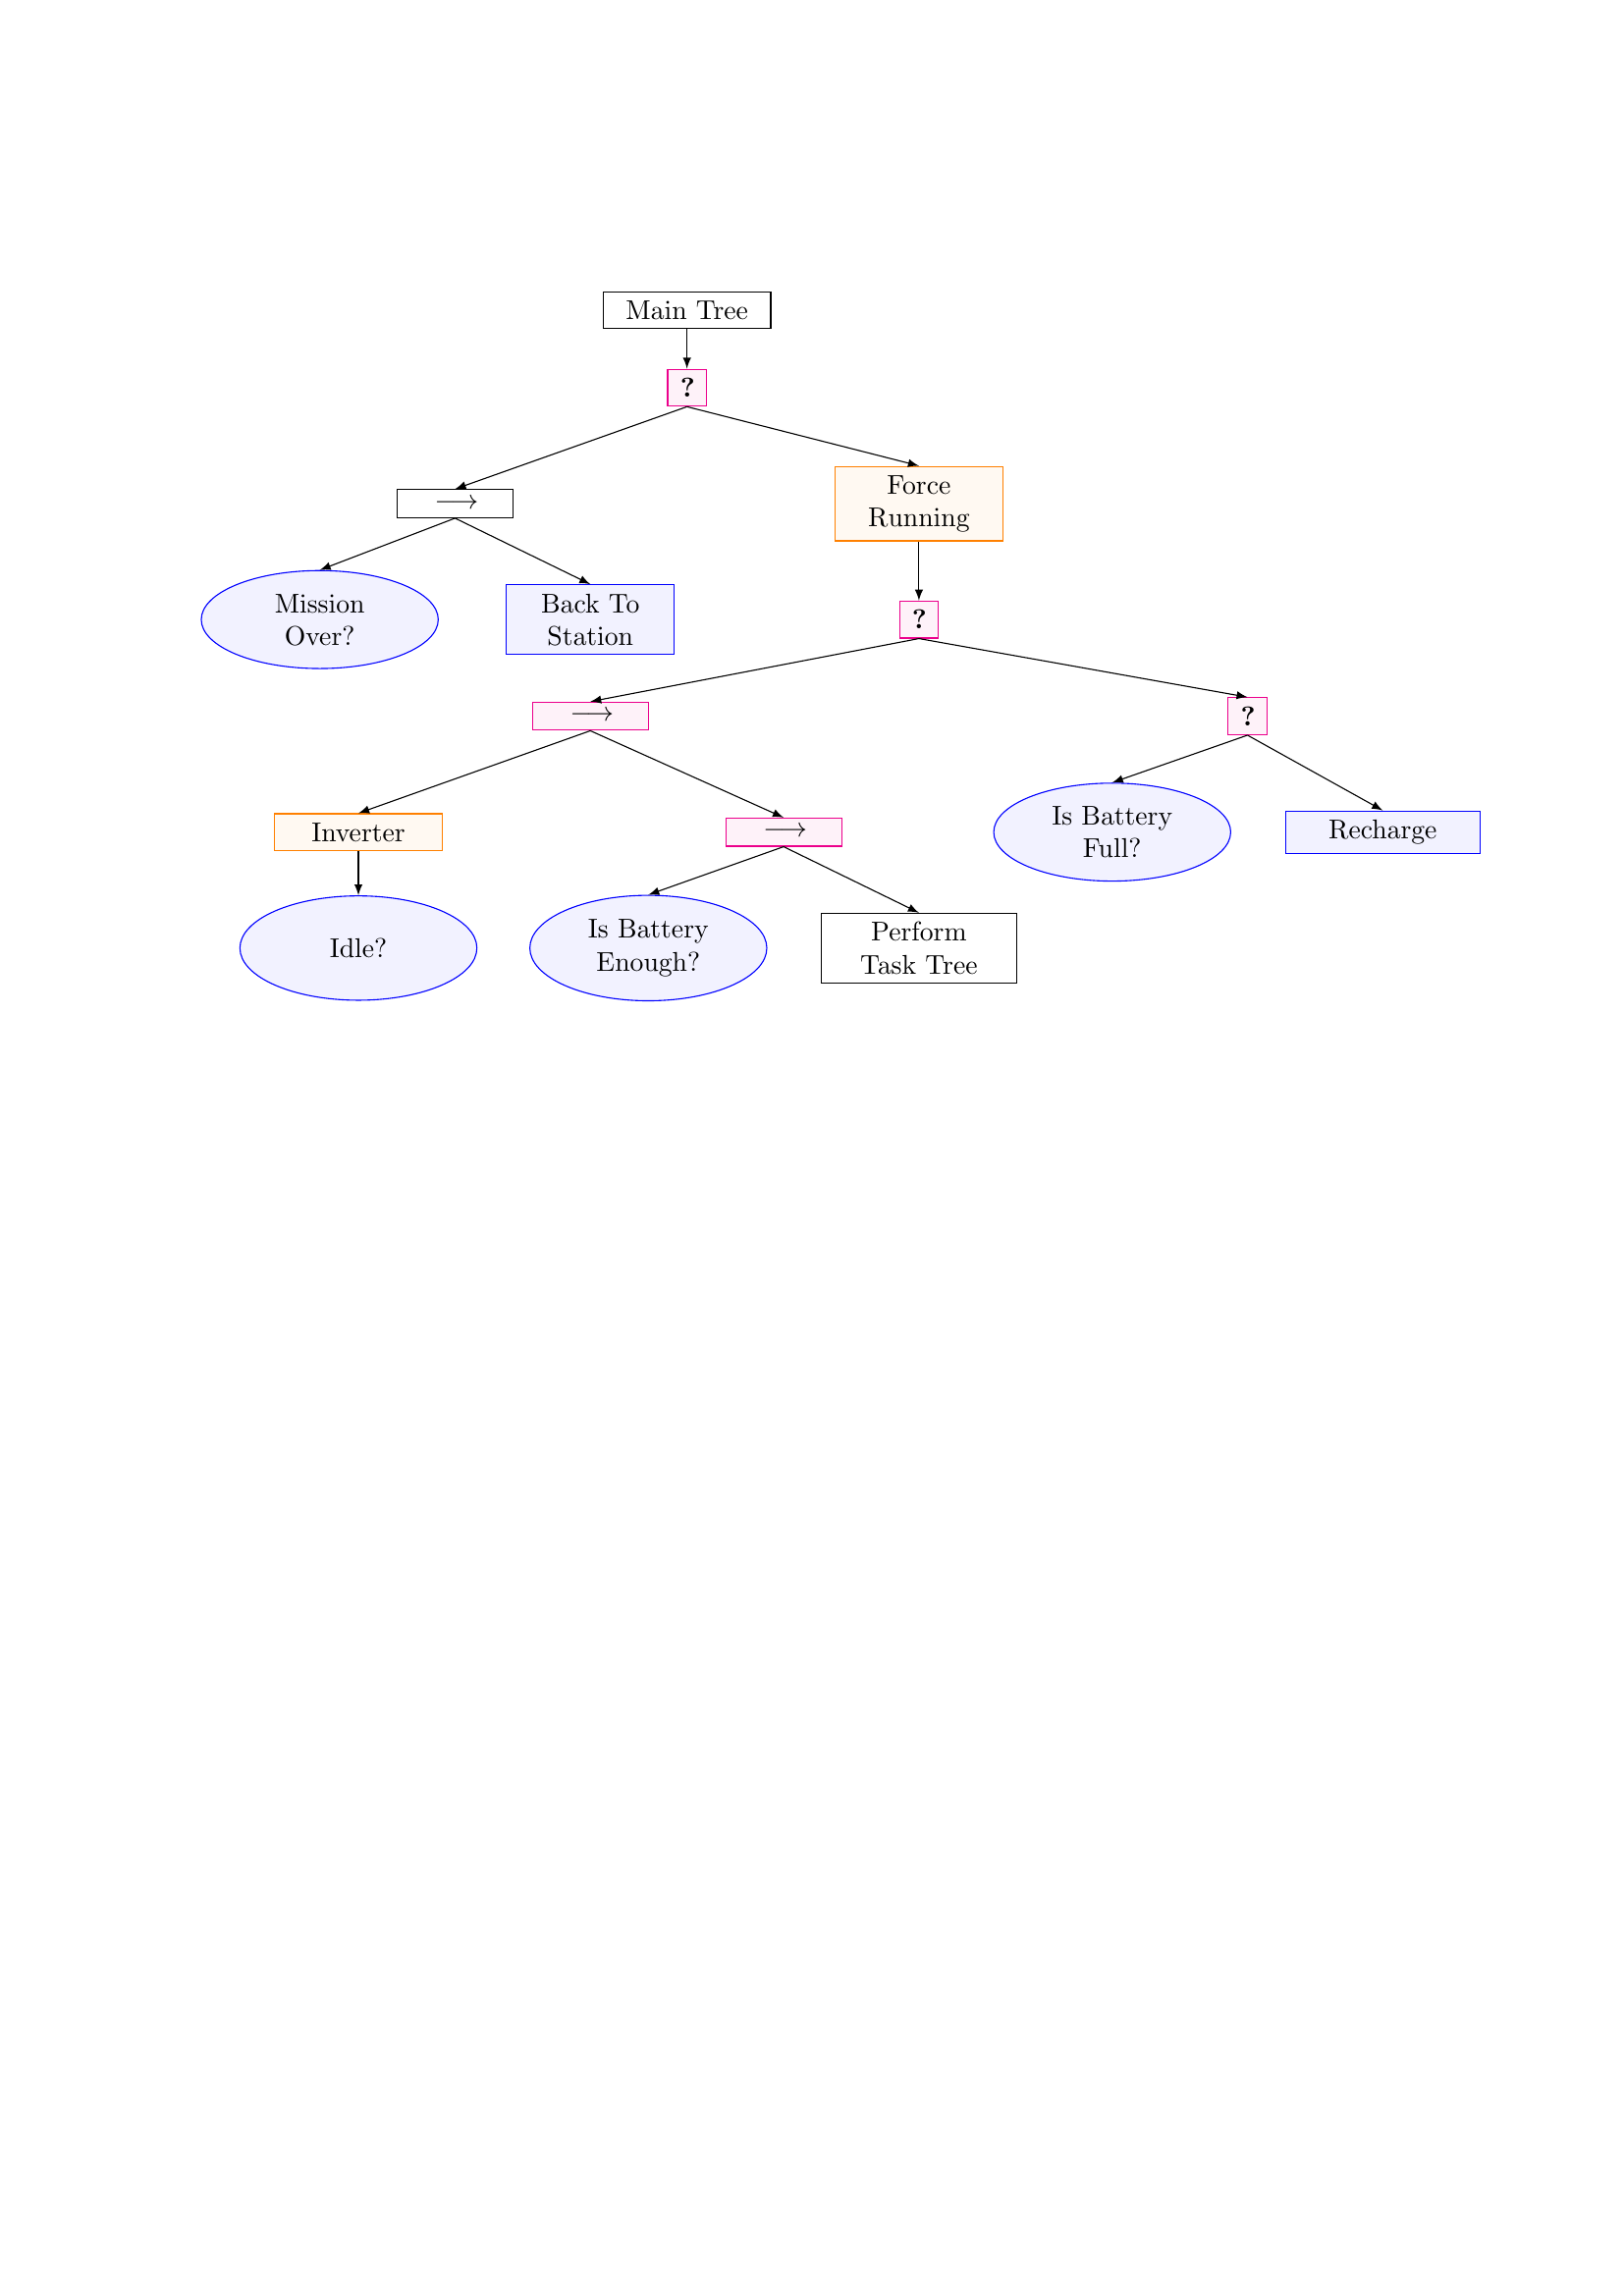
\begin{tikzpicture}
        		\node (MainTree) at (0,0) [text centered, fill=white, draw, rectangle, minimum width=1.5cm, text width=5.5em]{Main Tree};

        		\node (RootFallback) at ($(MainTree) + (0,-1)$) [text centered, fill=magenta!5, draw=magenta, rectangle, minimum width=0.5cm, text width=0.5em]{\textbf{?}};
        		\draw[-latex] (MainTree.south) -- (RootFallback.north);

        		\node (MissionOverSequence) at ($(RootFallback) + (-3,-1.5)$) [text centered, fill=white, draw, rectangle, minimum width=1.5cm, text width=1.5em]{$\longrightarrow$};
        		\draw[-latex] (RootFallback.south) -- (MissionOverSequence.north);
        		\node (ForceRunning) at ($(RootFallback) + (3, -1.5)$) [text centered, fill=orange!5, draw=orange, rectangle, minimum width=1.5cm, text width=5.5em]{Force Running};
        		\draw[-latex] (RootFallback.south) -- (ForceRunning.north);
        		
        		\node (MissionOver) at ($(MissionOverSequence) + (-1.75,-1.5)$) [text centered, fill=blue!5, draw=blue, ellipse, minimum width=1.5cm, text width=5.5em]{Mission Over?};
        		\draw[-latex] (MissionOverSequence.south) -- (MissionOver.north);
        		\node (BackToStation) at ($(MissionOverSequence) + (1.75, -1.5)$) [text centered, fill=blue!5, draw=blue, rectangle, minimum width=1.5cm, text width=5.5em]{Back To Station};
        		\draw[-latex] (MissionOverSequence.south) -- (BackToStation.north);
        		\node (MissionFallback) at ($(ForceRunning) + (0,-1.5)$) [text centered, fill=magenta!5, draw=magenta, rectangle, minimum width=0.5cm, text width=0.5em]{\textbf{?}};
        		\draw[-latex] (ForceRunning.south) -- (MissionFallback.north);

        		\node (IdleSequence) at ($(MissionFallback) + (-4.25,-1.25)$) [text centered, fill=magenta!5, draw=magenta, rectangle, minimum width=1.5cm, text width=1.5em]{$\longrightarrow$};
        		\draw[-latex] (MissionFallback.south) -- (IdleSequence.north);
        		\node (WaitFallback) at ($(MissionFallback) + (4.25,-1.25)$) [text centered, fill=magenta!5, draw=magenta, rectangle, minimum width=0.5cm, text width=0.5em]{\textbf{?}};
        		\draw[-latex] (MissionFallback.south) -- (WaitFallback.north);
        		
        		\node (Inverter) at ($(IdleSequence) + (-3, -1.5)$) [text centered, fill=orange!5, draw=orange, rectangle, minimum width=1.5cm, text width=5.5em]{Inverter};
        		\draw[-latex] (IdleSequence.south) -- (Inverter.north);
        		\node (TaskSequence) at ($(IdleSequence) + (2.5,-1.5)$) [text centered, fill=magenta!5, draw=magenta, rectangle, minimum width=1.5cm, text width=1.5em]{$\longrightarrow$};
        		\draw[-latex] (IdleSequence.south) -- (TaskSequence.north);
        		\node (IsBatteryFull) at ($(WaitFallback) + (-1.75,-1.5)$) [text centered, fill=blue!5, draw=blue, ellipse, minimum width=1.5cm, text width=5.5em]{Is Battery Full?};
        		\draw[-latex] (WaitFallback.south) -- (IsBatteryFull.north);
        		\node (Recharge) at ($(WaitFallback) + (1.75, -1.5)$) [text centered, fill=blue!5, draw=blue, rectangle, minimum width=1.5cm, text width=6.5em]{Recharge};
        		\draw[-latex] (WaitFallback.south) -- (Recharge.north);

        		\node (Idle) at ($(Inverter) + (0,-1.5)$) [text centered, fill=blue!5, draw=blue, ellipse, minimum width=1.5cm, minimum height=1.35cm, text width=5.5em]{Idle?};
        		\draw[-latex] (Inverter.south) -- (Idle.north);
        		\node (IsBatteryEnough) at ($(TaskSequence) + (-1.75,-1.5)$) [text centered, fill=blue!5, draw=blue, ellipse, minimum width=1.5cm, text width=5.5em]{Is Battery Enough?};
        		\draw[-latex] (TaskSequence.south) -- (IsBatteryEnough.north);
        		\node (PerformTaskTree) at ($(TaskSequence) + (1.75, -1.5)$) [text centered, fill=white, draw, rectangle, minimum width=1.5cm, text width=6.5em]{Perform Task Tree};
        		\draw[-latex] (TaskSequence.south) -- (PerformTaskTree.north);
        		
        		%\draw[-latex] (.south) -- (.north);
		    \end{tikzpicture}}
		\caption{Árbol de comportamiento: Árbol principal}
		\label{fig:MainTree}
	\end{center}
	\vspace{-1em}
\end{figure}

Este \gls{BT} comprueba si la misión ha terminado y si es así dirige el \gls{ACW} de vuelta a la estación base. Si no es así se comprueba si hay alguna tarea asignada. Si resulta que el \gls{ACW} está ocioso y la batería no está al cien por cien, el \gls{ACW} es guiado a una estación de recarga (aquí es donde está codificado el protocolo de emergencia). Si se asigna una tarea y la batería es suficiente, se entra en el \emph{Árbol de ejecutar tarea} (subárbol representado en la Figura~\ref{fig:PerformTasksTree}).

\begin{figure}[ht]
	\begin{center}
		\scalebox{0.75}{
			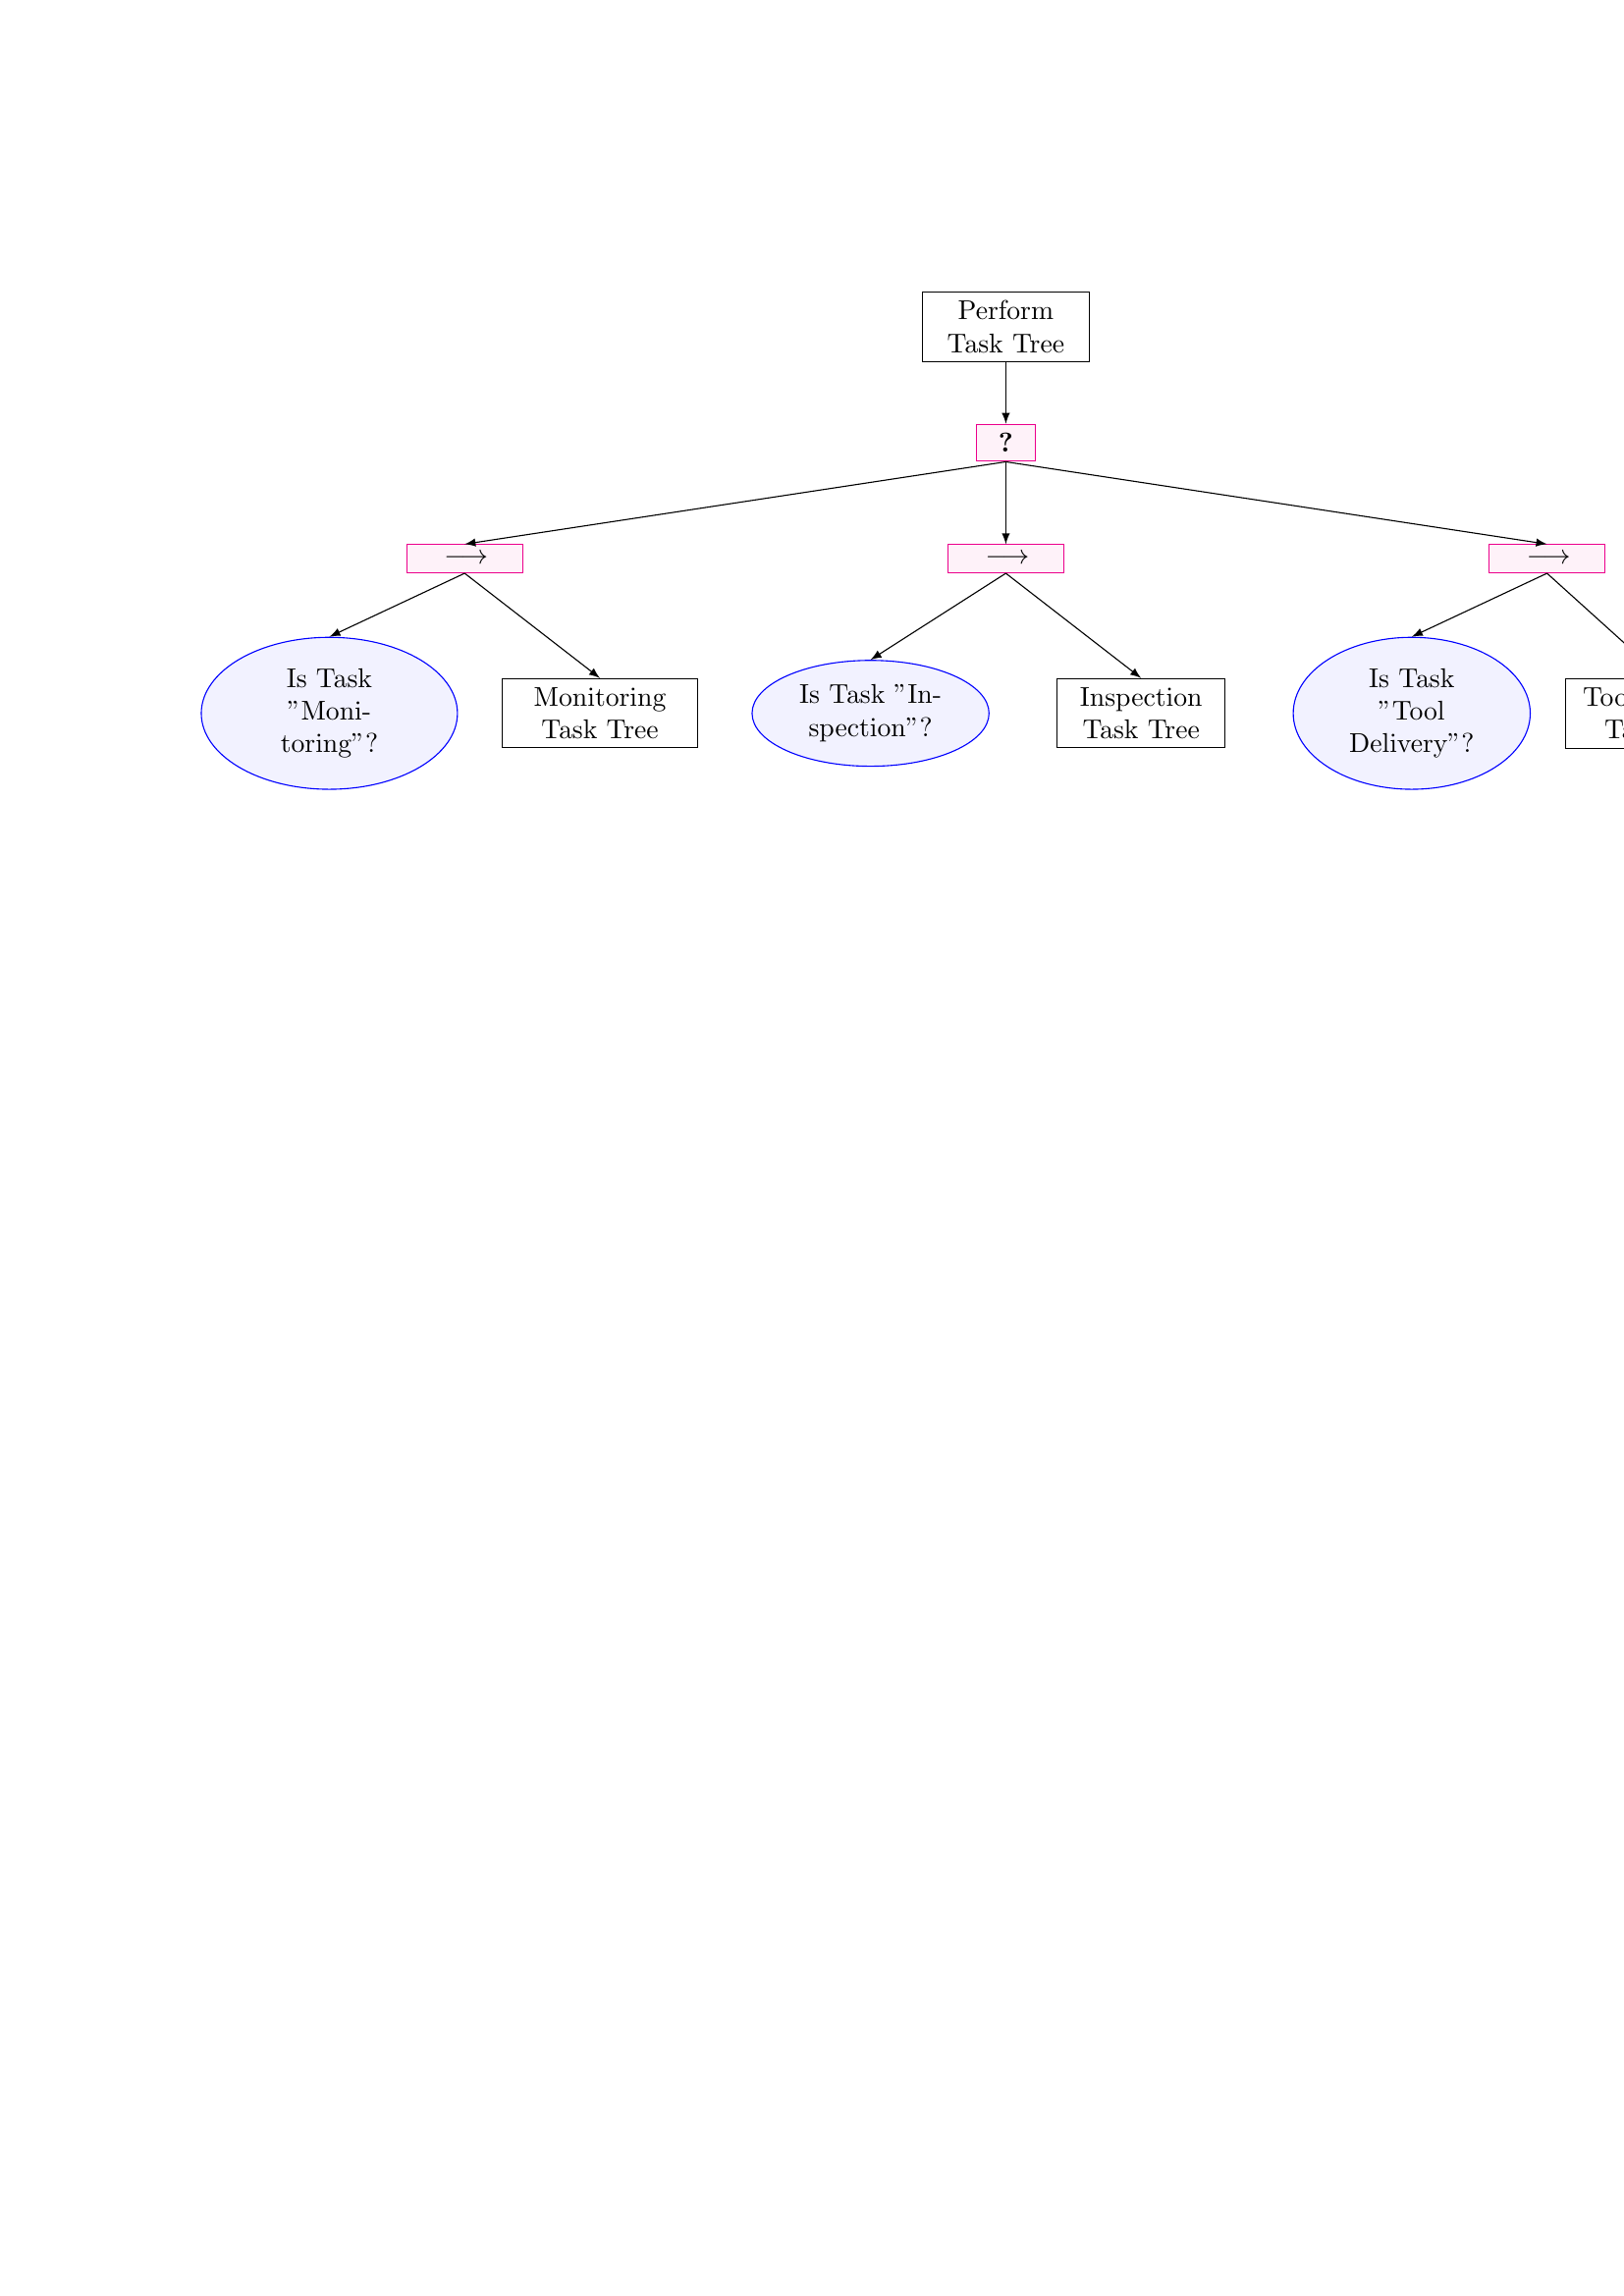
\begin{tikzpicture}
			    \node (PerformTaskTree) at (0,0) [text centered, fill=white, draw, rectangle, minimum width=1.5cm, text width=5.5em]{Perform Task Tree};
        		
        		\node (TaskFallback) at ($(PerformTaskTree) + (0,-1.5)$) [text centered, fill=magenta!5, draw=magenta, rectangle, minimum width=0.5cm, text width=1.5em]{\textbf{?}};
        		\draw[-latex] (PerformTaskTree.south) -- (TaskFallback.north);
        		
        		\node (MonitorSequence) at ($(TaskFallback) + (-7,-1.5)$) [text centered, fill=magenta!5, draw=magenta, rectangle, minimum width=1.5cm, text width=1.5em]{$\longrightarrow$};
        		\draw[-latex] (TaskFallback.south) -- (MonitorSequence.north);
        		\node (InspectSequence) at ($(TaskFallback) + (0,-1.5)$) [text centered, fill=magenta!5, draw=magenta, rectangle, minimum width=1.5cm, text width=1.5em]{$\longrightarrow$};
        		\draw[-latex] (TaskFallback.south) -- (InspectSequence.north);
        		\node (DeliverSequence) at ($(TaskFallback) + (7,-1.5)$) [text centered, fill=magenta!5, draw=magenta, rectangle, minimum width=1.5cm, text width=1.5em]{$\longrightarrow$};
        		\draw[-latex] (TaskFallback.south) -- (DeliverSequence.north);
        		
        		\node (IsTaskMonitor) at ($(MonitorSequence) + (-1.75,-2)$) [text centered, fill=blue!5, draw=blue, ellipse, minimum width=1.5cm, text width=6em]{Is Task "Monitoring"?};
        		\draw[-latex] (MonitorSequence.south) -- (IsTaskMonitor.north);
        		\node (MonitorTree) at ($(MonitorSequence) + (1.75, -2)$) [text centered, fill=white, draw, rectangle, minimum width=1.5cm, text width=6.5em]{Monitoring Task Tree};
        		\draw[-latex] (MonitorSequence.south) -- (MonitorTree.north);
        		\node (IsTaskInspect) at ($(InspectSequence) + (-1.75,-2)$) [text centered, fill=blue!5, draw=blue, ellipse, minimum width=1.5cm, text width=5.5em]{Is Task "Inspection"?};
        		\draw[-latex] (InspectSequence.south) -- (IsTaskInspect.north);
        		\node (InspectTree) at ($(InspectSequence) + (1.75, -2)$) [text centered, fill=white, draw, rectangle, minimum width=1.5cm, text width=5.5em]{Inspection Task Tree};
        		\draw[-latex] (InspectSequence.south) -- (InspectTree.north);
        		\node (IsTaskDeliver) at ($(DeliverSequence) + (-1.75,-2)$) [text centered, fill=blue!5, draw=blue, ellipse, minimum width=1.5cm, text width=5.5em]{Is Task "Tool Delivery"?};
        		\draw[-latex] (DeliverSequence.south) -- (IsTaskDeliver.north);
        		\node (DeliverTree) at ($(DeliverSequence) + (1.5, -2)$) [text centered, fill=white, draw, rectangle, minimum width=1.5cm, text width=6.5em]{Tool Delivery Task Tree};
        		\draw[-latex] (DeliverSequence.south) -- (DeliverTree.north);
        		
		    \end{tikzpicture}}
		\caption{Árbol de comportamiento: Árbol de ejecutar tarea}
		\label{fig:PerformTasksTree}
	\end{center}
\end{figure}

El \emph{Árbol de ejecutar tarea} comprueba cuál es la primera tarea de la cola, que es la que debe ejecutarse en ese momento. En las figuras \ref{fig:MonitorTree}, \ref{fig:InspectTree} y \ref{fig:DeliverToolTree} se representan los subárboles que ejecutan las tareas. Se decidió que el control total no se daría a los controladores de bajo nivel hasta que el \gls{ACW} estuviera lo suficientemente cerca de la zona donde se desarrolla la tarea.

\subsection{Árbol de la tarea inspección}
\label{sec:InspectionTaskTree}
Este \gls{BT} es bastante sencillo, ya que la tarea consiste simplemente en visitar una serie de puntos y detenerse en cada uno de ellos para tomar fotografías (véase la \ref{fig:InspectTree}). El BT omprueba si el \gls{ACW} está cerca de los puntos a inspeccionar, si es necesario, se ejecuta el nodo para ir cerca de \gls{WP} y una vez allí, se llama al controlador de bajo nivel que ejecuta esta tarea.

\begin{figure}[ht]
	\begin{center}
		\scalebox{0.9}{
			\begin{tikzpicture}
			    \node (InspectTree) at (0,0) [text centered, fill=white, draw, rectangle, minimum width=1.5cm, text width=5.5em]{Inspection Task Tree};
        		
        		\node (InspectTaskSequence) at ($(InspectTree) + (0,-1.5)$) [text centered, fill=magenta!5, draw=magenta, rectangle, minimum width=1.5cm, text width=1.5em]{$\longrightarrow$};
        		\draw[-latex] (InspectTree.south) -- (InspectTaskSequence.north);
        		
        		\node (NearWPFallback) at ($(InspectTaskSequence) + (-1.5,-1.5)$) [text centered, fill=magenta!5, draw=magenta, rectangle, minimum width=0.5cm, text width=0.5em]{\textbf{?}};
        		\draw[-latex] (InspectTaskSequence.south) -- (NearWPFallback.north);
        		\node (Inspect) at ($(InspectTaskSequence) + (1.5,-1.5)$) [text centered, fill=blue!5, draw=blue, rectangle, minimum width=1.5cm, text width=5.5em]{Inspect};
        		\draw[-latex] (InspectTaskSequence.south) -- (Inspect.north);
        		
        		\node (IsUAVnearWP) at ($(NearWPFallback) + (-1.75,-2)$) [text centered, fill=blue!5, draw=blue, ellipse, minimum width=1.5cm, text width=5.5em]{Is \gls{ACW} near WP?};
        		\draw[-latex] (NearWPFallback.south) -- (IsUAVnearWP.north);
        		\node (GoNearWP) at ($(NearWPFallback) + (1.75, -2)$) [text centered, fill=blue!5, draw=blue, rectangle, minimum width=1.5cm, text width=6.5em]{Go near WP};
        		\draw[-latex] (NearWPFallback.south) -- (GoNearWP.north);
		    \end{tikzpicture}}
		\caption{Árbol de comportamiento: sub-arbol que controla las tareas de inspección}
		\label{fig:InspectTree}
	\end{center}
\end{figure}

\subsection{Árbol de la tarea de monitorización}
\label{sec:MonitoringTaskTree}
Como se puede ver en la Figura \ref{fig:MonitorTree}, este \gls{BT} sigue la misma estructura y funcionamiento que el anterior. Las únicas diferencias son los nodos \emph{Hoja}.

\begin{figure}[ht]
	\begin{center}
		\scalebox{0.9}{
			\begin{tikzpicture}
			    \node (MonitorTree) at (0,0) [text centered, fill=white, draw, rectangle, minimum width=1.5cm, text width=5.5em]{Monitoring Task Tree};
        		
        		\node (MonitorTaskSequence) at ($(MonitorTree) + (0,-1.5)$) [text centered, fill=magenta!5, draw=magenta, rectangle, minimum width=1.5cm, text width=1.5em]{$\longrightarrow$};
        		\draw[-latex] (MonitorTree.south) -- (MonitorTaskSequence.north);
        		
        		\node (NearHumanFallback) at ($(MonitorTaskSequence) + (-1.5,-1.5)$) [text centered, fill=magenta!5, draw=magenta, rectangle, minimum width=0.5cm, text width=1.5em]{\textbf{?}};
        		\draw[-latex] (MonitorTaskSequence.south) -- (NearHumanFallback.north);
        		\node (MonitorHumanTarget) at ($(MonitorTaskSequence) + (1.5,-1.5)$) [text centered, fill=blue!5, draw=blue, rectangle, minimum width=1.5cm, text width=5.5em]{Monitor};
        		\draw[-latex] (MonitorTaskSequence.south) -- (MonitorHumanTarget.north);
        		
        		\node (IsUAVnearHumanTarget) at ($(NearHumanFallback) + (-2,-2)$) [text centered, fill=blue!5, draw=blue, ellipse, minimum width=1.5cm, text width=6.5em]{Is \gls{ACW} near Human Target?};
        		\draw[-latex] (NearHumanFallback.south) -- (IsUAVnearHumanTarget.north);
        		\node (GoNearHuman) at ($(NearHumanFallback) + (1.55, -2)$) [text centered, fill=blue!5, draw=blue, rectangle, minimum width=1.5cm, text width=6.5em]{Go near Human Target};
        		\draw[-latex] (NearHumanFallback.south) -- (GoNearHuman.north);
		    \end{tikzpicture}}
		\caption{Árbol de comportamiento: sub-arbol que controla las tareas de monitorización}
		\label{fig:MonitorTree}
	\end{center}
	\vspace{-1em}
\end{figure}

\subsection{Árbol de la tarea de entrega de herramienta}
\label{sec:ToolDeliveryTaskTree}
Este árbol es un poco más complejo, ya que la tarea implica varios pasos (ver Fig. \ref{fig:DeliverToolTree}). En primer lugar, recoge la herramienta solicitada en caso de que el \gls{ACW} no la tenga todavía, luego se realiza la aproximación al operario, y por último el controlador de bajo nivel de esta tarea puede ser activado.

\begin{figure}[ht]
	\begin{center}
		\scalebox{0.85}{
			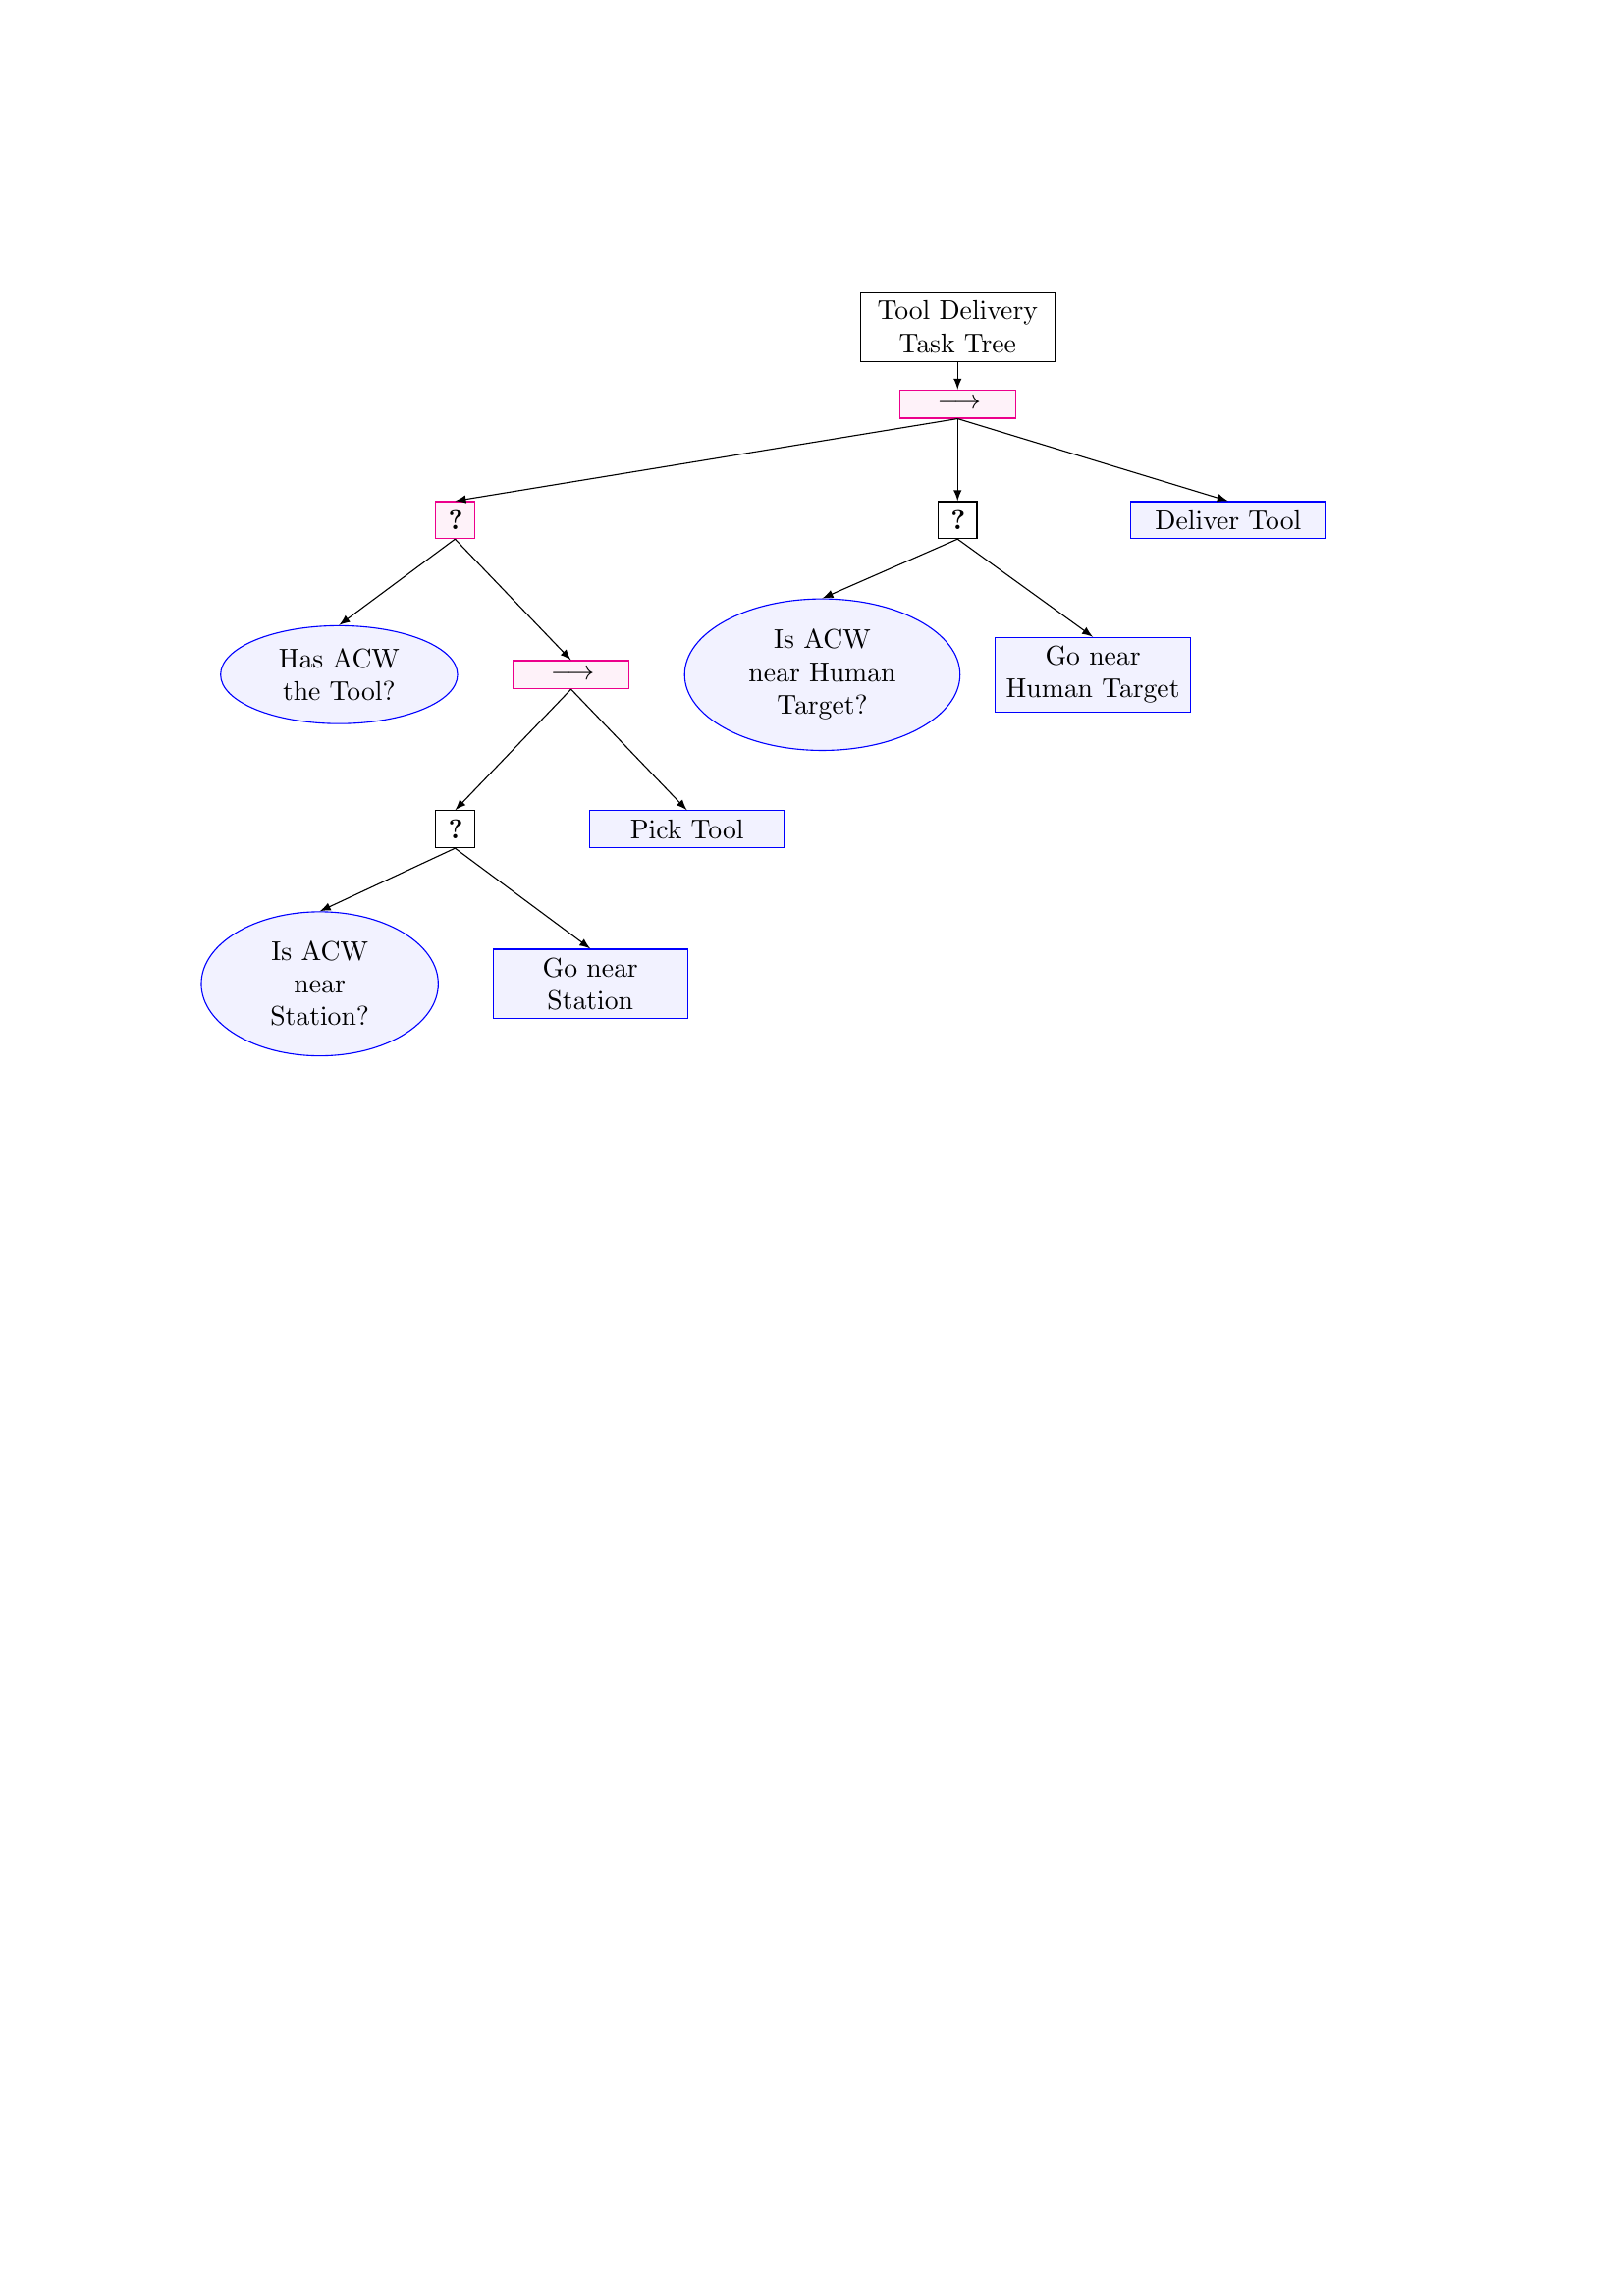
\begin{tikzpicture}
			    \node (DeliverTree) at (0,0) [text centered, fill=white, draw, rectangle, minimum width=1.5cm, text width=6.5em]{Tool Delivery Task Tree};
			    
			    \node (DeliverTaskSequence) at ($(DeliverTree) + (0,-1)$) [text centered, fill=magenta!5, draw=magenta, rectangle, minimum width=1.5cm, text width=1.5em]{$\longrightarrow$};
        		\draw[-latex] (DeliverTree.south) -- (DeliverTaskSequence.north);

				\node (ToolFallback) at ($(DeliverTaskSequence) + (-6.5,-1.5)$) [text centered, fill=magenta!5, draw=magenta, rectangle, minimum width=0.5cm, text width=0.5em]{\textbf{?}};
        		\draw[-latex] (DeliverTaskSequence.south) -- (ToolFallback.north);
        		\node (HumanFallback) at ($(DeliverTaskSequence) + (0,-1.5)$) [text centered, fill=white, draw, rectangle, minimum width=0.5cm, text width=0.5em]{\textbf{?}};
        		\draw[-latex] (DeliverTaskSequence.south) -- (HumanFallback.north);
        		%\node (PermissionFallback) at ($(DeliverTaskSequence) + (6.5,-1.5)$) [text centered, fill=magenta!5, draw=magenta, rectangle, minimum width=0.5cm, text width=0.5em]{\textbf{?}};
        		%\draw[-latex] (DeliverTaskSequence.south) -- (PermissionFallback.north);
				\node (DeliverTool) at ($(DeliverTaskSequence) + (3.5,-1.5)$) [text centered, fill=blue!5, draw=blue, rectangle, minimum width=1.5cm, text width=6.5em]{Deliver Tool};
        		\draw[-latex] (DeliverTaskSequence.south) -- (DeliverTool.north);

				\node (hasACWtheTool) at ($(ToolFallback) + (-1.5,-2)$) [text centered, fill=blue!5, draw=blue, ellipse, minimum width=1.5cm, text width=5.5em]{Has \gls{ACW} the Tool?};
        		\draw[-latex] (ToolFallback.south) -- (hasACWtheTool.north);
        		\node (PickToolSequence) at ($(ToolFallback) + (1.5,-2)$) [text centered, fill=magenta!5, draw=magenta, rectangle, minimum width=1.5cm, text width=1.5em]{$\longrightarrow$};
        		\draw[-latex] (ToolFallback.south) -- (PickToolSequence.north);
        		\node (IsUAVnearHuman) at ($(HumanFallback) + (-1.75,-2)$) [text centered, fill=blue!5, draw=blue, ellipse, minimum width=1.5cm, text width=6.5em]{Is \gls{ACW} near Human Target?};
        		\draw[-latex] (HumanFallback.south) -- (IsUAVnearHuman.north);
        		\node (GoNearHuman) at ($(HumanFallback) + (1.75, -2)$) [text centered, fill=blue!5, draw=blue, rectangle, minimum width=1.5cm, text width=6.5em]{Go near Human Target};
        		\draw[-latex] (HumanFallback.south) -- (GoNearHuman.north);
        		%\node (DeliverSequence) at ($(PermissionFallback) + (-2.25,-2)$) [text centered, fill=white, draw, rectangle, minimum width=1.5cm, text width=1.5em]{$\longrightarrow$};
        		%\draw[-latex] (PermissionFallback.south) -- (DeliverSequence.north);
        		%\node (ForceFailure) at ($(PermissionFallback) + (2.25, -2)$) [text centered, fill=orange!5, draw=orange, rectangle, minimum width=1.5cm, text width=5.5em]{Force Failure};
        		%\draw[-latex] (PermissionFallback.south) -- (ForceFailure.north);


        		\node (StationFallback) at ($(PickToolSequence) + (-1.5,-2)$) [text centered, fill=white, draw, rectangle, minimum width=0.5cm, text width=0.5em]{\textbf{?}};
        		\draw[-latex] (PickToolSequence.south) -- (StationFallback.north);
        		\node (PickTool) at ($(PickToolSequence) + (1.5, -2)$) [text centered, fill=blue!5, draw=blue, rectangle, minimum width=1.5cm, text width=6.5em]{Pick Tool};
        		\draw[-latex] (PickToolSequence.south) -- (PickTool.north);
        		%\node (hasUAVpermission) at ($(DeliverSequence) + (-3.25,-2)$) [text centered, fill=white, draw, ellipse, minimum width=1.5cm, text width=5.5em]{Has  permission?};
        		%\draw[-latex] (DeliverSequence.south) -- (hasUAVpermission.north);
        		%\node (DeliverTool) at ($(DeliverSequence) + (0, -2)$) [text centered, fill=white, draw, rectangle, minimum width=1.5cm, text width=6.5em]{Tool Delivery};
        		%\draw[-latex] (DeliverSequence.south) -- (DeliverTool.north);
        		%\node (Retreat) at ($(DeliverSequence) + (3, -2)$) [text centered, fill=white, draw, rectangle, minimum width=1.5cm, text width=4.5em]{Retreat};
        		%\draw[-latex] (DeliverSequence.south) -- (Retreat.north);
        		%\node (WaitFallback) at ($(ForceFailure) + (0,-2)$) [text centered, fill=magenta!5, draw=magenta, rectangle, minimum width=0.5cm, text width=0.5em]{\textbf{?}};
        		%\draw[-latex] (ForceFailure.south) -- (WaitFallback.north);
        		
        		\node (IsUAVnearStation) at ($(StationFallback) + (-1.75,-2)$) [text centered, fill=blue!5, draw=blue, ellipse, minimum width=1.5cm, text width=5.5em]{Is \gls{ACW} near Station?};
        		\draw[-latex] (StationFallback.south) -- (IsUAVnearStation.north);
        		\node (GoNearStation) at ($(StationFallback) + (1.75, -2)$) [text centered, fill=blue!5, draw=blue, rectangle, minimum width=1.5cm, text width=6.5em]{Go near Station};
        		\draw[-latex] (StationFallback.south) -- (GoNearStation.north);
        		%\node (TimeoutSequence) at ($(WaitFallback) + (-1.5,-2)$) [text centered, fill=white, draw, rectangle, minimum width=1.5cm, text width=1.5em]{$\longrightarrow$};
        		%\draw[-latex] (WaitFallback.south) -- (TimeoutSequence.north);
        		%\node (Wait) at ($(WaitFallback) + (1.5, -2)$) [text centered, fill=white, draw, rectangle, minimum width=1.5cm, text width=6.5em]{Wait for Permission};
        		%\draw[-latex] (WaitFallback.south) -- (Wait.north);

        		%\node (Timeout) at ($(TimeoutSequence) + (-3.25,-2)$) [text centered, fill=white, draw, ellipse, minimum width=1.5cm, text width=5.5em]{Timeout?};
        		%\draw[-latex] (TimeoutSequence.south) -- (Timeout.north);
        		%\node (GoNearStation) at ($(TimeoutSequence) + (0, -2)$) [text centered, fill=white, draw, rectangle, minimum width=1.5cm, text width=6.5em]{Go near Station};
        		%\draw[-latex] (TimeoutSequence.south) -- (GoNearStation.north);
        		%\node (DropTool) at ($(TimeoutSequence) + (3.25, -2)$) [text centered, fill=white, draw, rectangle, minimum width=1.5cm, text width=6.5em]{Drop the Tool};
        		%\draw[-latex] (TimeoutSequence.south) -- (DropTool.north);
		    \end{tikzpicture}}
		\caption{Árbol de comportamiento: sub-árbol que controla la tarea de entrega de herramienta}
		\label{fig:DeliverToolTree}
	\end{center}
\end{figure}

%\section{High- and low-level blocks faking}
%\label{sec:faking}
%The work in this thesis consisted of programming one of the software layers that make up a software architecture. As there are still parts of the software architecture that are not yet available for integration, temporary solutions have had to be programmed to simulate their action during testing. This section will discuss those parts of the code whose mission is to fool both \emph{High-Level Planner} and \emph{Agent Behaviour Manager} blocks into believing that they are communicating with the real blocks, or to provide functions necessary for the execution to progress.

%Low-level controllers have been faked in different ways. For \gls{BT}'s \emph{Action} nodes of the \emph{"Go To"} type, the \emph{GoToWaypoint} \gls{ROS} service available in the \gls{UAL} tool is called instead, which leads the \gls{UAV} to the entered coordinates (although it does not take obstacles into account). For more complex \emph{Action} nodes such as \emph{Inspect}, \emph{Monitor}, \emph{Deliver Tool} or \emph{Pick Tool}, a function is simply called which sleeps the \emph{Action} node for a while simulating that the low-level controller has been called and is waiting for a response. For these \emph{Action} nodes, the response of the \emph{tick} function will be \emph{RUNNING} while sleeping, and either \emph{FAILURE} or \emph{SUCCESS} depending on whether their execution is halted or not. During sleeping time the rest of the tree continues running. The \emph{Recharge} node also calls some low-level controllers. In this particular case it was decided to ignore the call and simply land the \gls{UAV} on the charging station.

%On the other hand, since \gls{UAL} does not allow battery control, and the battery level that is available for reading remains static throughout the simulation, it has been necessary to create a block that simulates the evolution of the battery both during flight and during recharging. This block is programmed in such a way that at initialisation it reads the configuration file, thus having the position of the charging stations, and also subscribes to the information published by the \emph{\gls{ACW}'s autopilot} to which it is faking the battery in order to know its position and status. If the \gls{UAV} is in the air, the battery will be periodically decremented. Otherwise, the battery will remain static unless the \gls{UAV} is over a charging station, in which case the battery will periodically increment. The battery percentage and charge/discharge rate is externally configurable at any time during the simulation. In addition, for ease of testing, this block allows for different modes of operation that can among other things make the battery static. The false battery level is periodically published in a similar direction to the one used for the real battery.

%Finally, as mentioned in the section \ref{sec:Centralised module:TaskPlanner}, the algorithm in charge of performing the distribution of \glspl{WP} for an inspection task among the different selected \glspl{ACW} has been forged. Normally, this algorithm is executed inside the low-level controller itself which is called by the \emph{Inspect Action} node which can be found in the tree of the figure \ref{fig:InspectTree}. However, as this \emph{Action} node has been completely forged, a distribution of \glspl{WP} has been made within the task planning algorithm. It simply assigns, in order, one \gls{WP} from the list to each selected \gls{ACW} until the list of \glspl{WP} is exhausted.
%
%\chapter{Results}
\label{ch:Results}

\lettrine[lraise=-0.1, lines=2, loversize=0.2]{L}{o}rem itsum

\section{Task planning}
\label{sec:TaskPlanning}

\subsection{Battery}
\label{subsec:Battery}

\subsection{Connection lost}
\label{subsec:ConnectionLost}

\subsection{Replanning}
\label{subsec:Replanning}


\section{Drone behaviour manager results}
\label{sec:DroneBehavioutManagerResults}

\subsection{Battery management}
\label{subsec:BatteryManagement}

\subsection{Connection lost management}
\label{subsec:ConnectionLostManagement}

\subsection{Replanning management}
\label{subsec:ReplanningManagement}


\section{Simulations}
\label{sec:Simulations}

\subsection{One drone simulations}
\label{subsec:OneDroneSimulations}

\subsection{Multi-drone simulations}
\label{subsec:Multi-droneSimulations}


\chapter{Results}
\label{ch:Results}
\lettrine[lraise=-0.1, lines=2, loversize=0.2]{E}{n} este capítulo se exponen los experimentos realizados para validar la capa de software construida. Los experimentos se dividieron en dos fases. En la primera fase, se realizaron simulaciones con un solo \gls{ACW} para probar el rendimiento de cada elemento del sistema de forma controlada. Por un lado, se comprobó que el \emph{Planificador de alto nivel} realizaba la planificación de la misión correctamente, asignando las tareas como se esperaba según las especificaciones y restricciones, y por otro lado, se comprobó que el \emph{Gestor de comportamiento} realizaba su función correctamente, tanto la ejecución de las tareas individuales como la capacidad de detectar y actuar en caso de imprevistos. Durante esta fase, la validación del bloque distribuido cobra protagonismo. En la segunda fase, las simulaciones consistieron en incluir múltiples \glspl{ACW} y realizar pruebas en diferentes escenarios. Esta fase se centra menos en la validación del \gls{BT}, que estaría totalmente validado durante la primera fase, y más en la evaluación de las capacidades del \emph{Planificador de alto nivel}. Las situaciones a las que se enfrenta el sistema en esta fase implican desconexiones, reconexiones, entrada de nuevas tareas, modificaciones del nivel de batería, etc.

Los BTs funcionaron perfectamente. En Gazebo, se observó el movimiento de los \gls{ACW} de un lado a otro mientras los \gls{BT} recorrían los nodos del subárbol de cada tarea (ver Fig. \ref{fig:Gazebo_DeliverTree}). Además, se comprobó que el resultado de las tareas se comunicaba correctamente con el bloque centralizado.

\begin{figure}[htbp]
    \centering
    \subfloat[Posicion inicial: estación de carga]{
        \includegraphics[width=.3\linewidth]{Results/figures/GazeboBatSta.pdf}}
    \hfill
    \subfloat[Estación base: recogida de herramienta]{
        \includegraphics[width=.3\linewidth]{Results/figures/GazeboTool.pdf}}
    \hfill
    \subfloat[Posición del humano: entrega]{
        \includegraphics[width=.3\linewidth]{Results/figures/GazeboHuman.pdf}}
    \hfill
    \\
    \subfloat[Ir a la estacion]{
        \includegraphics[width=.45\linewidth]{Results/figures/BTDTGNS.pdf}}
    \hfill
    \subfloat[Recoger la herreamienta]{
        \includegraphics[width=.45\linewidth]{Results/figures/BTDTPT.pdf}}
    \\
    \subfloat[Ir al operario]{ 
        \includegraphics[width=.45\linewidth]{Results/figures/BTDTGNHT.pdf}}
    \hfill
    \subfloat[Entregar la herramienta]{
        \includegraphics[width=.45\linewidth]{Results/figures/BTDTDT.pdf}}
    \caption{Evolución de la simulación durante la ejecución de la tarea de entrega}
    \label{fig:Gazebo_DeliverTree}
\end{figure}

\begin{lstlisting}[caption={Mensajes impresos por el Gestor de comportamiento durante la ejecución del plan completo}, breaklines=true, label=exit:firstPlanFeedback]
    [ INFO][/uav_1/agent]: [newTaskList] Received a NewTaskList Action
    [ INFO][/uav_1/agent]: task_1: DeliverTool
    [ INFO][/uav_1/agent]: [Recharge] halt requested
    [ INFO][/uav_1/agent]: [GoNearStation] Moving near Tool...
    [ INFO][/uav_1/agent]: [PickTool] Calling Lower-level controllers...
    [ INFO][/uav_1/agent]: [PickTool] PICK TOOL FINISHED
    [ INFO][/uav_1/agent]: [GoNearHumanTarget] Moving near HT...
    [ INFO][/uav_1/agent]: [DeliverTool] Calling Lower-level controllers...
    [ INFO][/uav_1/agent]: [DeliverTool] DELIVER TOOL TASK FINISHED (true)
    [ INFO][/uav_1/agent]: task_2: Inspect
    [ INFO][/uav_1/agent]: [GoNearWP] Moving near WP...
    [ INFO][/uav_1/agent]: [TakeImage] Calling Lower-level controllers...
    [ INFO][/uav_1/agent]: [TakeImage] INSPECT TASK FINISHED (true)
    [ INFO][/uav_1/agent]: task_3: Monitor
    [ INFO][/uav_1/agent]: [GoNearHumanTarget] Moving near HT...
    [ INFO][/uav_1/agent]: [MonitorHumanTarget] Calling Lower-level controllers...
\end{lstlisting}

Una vez comprobado que el sistema funcionaba bien en ausencia de imprevistos, se probó el sistema en todo tipo de situaciones (capacidad del \gls{BT} para detener la tarea actual y pasar a la ejecución de la nueva tarea en caso de cambio de planes, llegada de una nueva tarea con un \gls{ID} repetido, pruebas de caída repentina de la batería, desconexiones, etc). El resultado de todas estas pruebas fue muy positivo. En la segunda fase se puso a prueba al planificador centralizado con cinco UAVs distintos y una gran variadad de situaciones tanto imprevistas como planificadas. Este bloque también superó con éxito todas las pruebas.

%
% \chapter{Conclusions and future work}
\label{ch:ConclusionsAndFutureWork}

\section{Conclusions}
\label{sec:Conclusions}
%% Comentar los objetivos marcados:
In this work, a task planning approach has been developed with the capability to perform mission planning for multi-\gls{UAV} teams. The system has sufficient cognitive capability to control multiple \glspl{UAV} operating as co-workers in dynamic environments safely. Simulations have demonstrated the system's ability to detect emergency situations and act in a safe way by executing contingency plans autonomously while calculating a new plan to follow that takes into account the unforeseen events that have occurred. The design of the system proposed two blocks: a centralised block on the ground in charge of optimal mission planning; and distributed blocks on board each of the \glspl{ACW} to allow the system to be robust to failures and have enough cognitive capacity to react to unforeseen events by recalculating the optimal plan. In this way, an efficient execution of tasks and a better use of resources is achieved, which translates into greater combined autonomy for the \gls{UAV} team.

The system has been designed in \gls{ROS} and the communications between the different software layers and the different blocks of each layer have been carried out using the tools offered by \gls{ROS}. This facilitates the integration of the system developed in other robotics projects that require a task planning system with these or similar characteristics. The use of \glspl{BT} for the design of the \gls{UAV} behaviour manager has great advantages over conventional \glspl{FSM}. This technique makes it possible to generate complex behaviours with numerous states without having to worry about taking into account each of the transitions between these states, as happens with \glspl{FSM}, in which the number of transitions grows exponentially with the number of states. The characteristics of the library used to program this part of the system make it easy to maintain, modify or extend. Moreover, thanks to its modular nature, this block can be reused in parts or in its entirety in any other project. The designed \gls{BT}, although it can be improved, has demonstrated in the simulations that works fairly well, laying the foundations for programming more complex behaviours in the future and serving as an example for the aerial robotics community, which can use it as a starting point for other applications. 

With respect to the block in charge of mission planning, the \emph{High-Level Planner}, it has so far demonstrated the ability to generate coherent plans in the conditions in which it has been tested and has also shown itself capable of recalculating these plans online in reaction to unforeseen events of different natures. The achieved solution is able to plan the mission taking into account imposed constraints such as the type of each \gls{ACW}, the priority of each of the tasks and the battery level of each of the \glspl{UAV}, being able to calculate plans for missions consisting of an indefinite number of tasks and \glspl{ACW}. Regarding the optimality of the plans generated by this block, it should be noticed that it has not been implemented any solution to approximate the optimal plan, but a heuristic solution based on a cost function that is calculated for each of the \glspl{ACW} with each of the tasks. However, this type of solution should be enough for initial tests in the targeted scenarios, are composed of few tasks and \glspl{ACW}. The solution reached, in this context, is a valid approximation towards a planning algorithm that generates a close-to-optimal plan.

\section{Future work}
\label{sec:FutureWork}
As part of the future work, the techniques developed in this work will be validated in a real environment with real \glspl{UAV}. In addition, the system will be used as a starting point for a PhD thesis in which it will be attempted to refine and improve the design of the \emph{Agent Behaviour Manager} block, as well as to develop a planning algorithm that generates a real approximation to the optimal plan for each situation. To this end, probabilistic decision-making algorithms will be introduced into the system, as well as the capacity to learn in real time some characteristics such as the \glspl{UAV}' battery consumption or human's intentions, thus anticipating unforeseen events and applying contingency plans. This would provide a greater robustness against failures and highly dynamic environments.

A first improvement for the planner with respect to the current version could be the incorporation of \emph{reload} tasks that, instead of being requested by human operators like the rest of the tasks, would be incorporated by the \emph{High-Level Planner} into the task queue, thus separating emergency reloads (or reloads that are executed when an agent is idle) from reloads carried out as part of the plan. Implementing this change in the \gls{BT} would mean modifying the \emph{Perform Task} tree to contemplate this new task in the design of the tree, a change that could be carried out by reusing and slightly adapting the trees used for the \emph{Inspection} and \emph{Safety Monitoring} tasks, taking advantage of the reusability of the \glspl{BT}.

In addition, in future work, it is intended to investigate the use of mixed reality technologies also for inspection applications with multi-\gls{UAV} teams, combining views taken from different points to recreate more complete visual environments for the operator, and improving the human-machine interaction of the system during collaborative tasks.

\endinput

\chapter{Conclusiones and trabajo futuro}
\label{ch:ConclusionsAndFutureWork}
\section{Conclusiones}
\label{sec:Conclusions}
En este trabajo se ha desarrolado un planificador de tareas con capacidad para realizar la planificación de misiones para equipos multi-UAV. El sistema tiene la capacidad cognitiva suficiente para controlar a múltiples UAVs que funcionen como co-trabajadores en entornos dinámicos de forma segura. Las simulaciones realizadas han demostrado la capacidad que tiene el sistema para detectar situaciones de emergencia y actuar de forma segura ejecutando planes de contingencia de forma autónoma mientras se calcula un nuevo plan a seguir que tenga en cuenta los imprevistos que hayan acontecido. El diseño del sistema dividido en un bloque centralizado en tierra encargado de realizar la planificación óptima de la misión y de bloques distribuidos a bordo de cada uno de los ACWs permite que el sistema presente robustez ante fallos y capacidad cognitiva suficiente para reaccionar ante eventos imprevistos recalculando el plan óptimo. De esta forma, se consigue una ejecución eficiente de las tareas y un mejor aprovechamiento de los recursos, que se traduce en una mayor autonomía conjunta del equipo de UAVs.

El sistema se ha diseñado en ROS y las comunicacioens entre las diferentes capas de software y los diferentes bloques de cada capa se han realizado empleando las herramientas que este ofrece. Esto facilita la integración del sistema desarrollado en otros proyectos de robótica que necesiten de un planificador de tareas con estas características o similares. El uso de BT para el diseño del UAV behaviour manager presenta grandes ventajas frente a las FSM convencionales. Esta técnica permite generar comportamientos complejos con numerosos estados sin que haya que preocuparse por tener en cuenta cada una de las transiciones entre esos estados como pasa con las FSM, en las que el número de transiciones crece exponencialmente con el número de estados. Las características de la librería empleada para programar esta parte del sistema hacen que sea facil de mantener, de modificar o de amplicar. Además, gracias a su caracter modular, este bloque puede ser reutilizado tanto a partes como en su totalidad en cualquier otro proyecto. El BT diseñado, aunque mejorable, ha demostrado en las simulaciones realizadas que funciona bastante bien, sentando las bases para programar comportamientos más complejos en el futuro y sirviendo de ejemplo para la comunidad de robótica aérea, que podrá emplearlo como punto de partida para otras aplicaciones. 

Respecto al bloque que se encarga de la planificación de la misión, el High-Level Planner, decir que hasta el momento ha demostrado tener la capacidad para general planes con sentido en las condiciones en las que se le ha puesto a prueba y que además ha demostrado ser capaz de recalcular dichos planes en línea como reacción a eventos imprevistos de diferente naturaleza. La solición alcanzada es capaz de planificar la misión teniento en cuenta resticciones impuestas como el tipo de cada ACW, la prioridad de cada una de las tareas y el nivel de autonomía de cada uno de los UAVs, siendo capaz de calcular planes para misiones formadas por una cantidad indefinida de tareas y ACWs. Respecto a la optimalidad de los planes generados por este bloque hay que decir que no se ha implementado ningún algoritmo que realice una búsqueda o aproximación del plan óptimo, sino que se ha diseñado una solución basada en una funcion de costes que se calcula para cada uno de los ACWs con cada una de las tareas. Sin embargo, este trabajo forma parte de un proyecto que tendrá aplicaciones reales en unas condiciones definidas. Por tanto, está justificado alejarse de análisis académicos en los que se busca aproximar el plan óptimo en misiones con un número indeterminado de tareas y de ACWs y analizar en su lugar al planificador en escenarios compuestos por pocas tareas y ACWs. La solución alcanzada, en este contexto, es una aproximación válida hacia un algoritmo de planificación que genere un plan próximo al óptimo.

\section{Trabajo futuro}
\label{sec:FutureWork}
Como parte del trabajo futuro se realizará una validación en un entorno real con equivos reales de las técnicas desarrolladas en este trabajo. Además, el sistema desarrollado en este trabajo se empleará como punto de partida de una tesis doctoral en la que se tratará de pulir y mejorar el diseño del Agent Behaviour Manager, así como de desarrollar un algoritmo de planificación que genere una aproximación real al plan óptimo de cada situación. Para ello se introducirán al sistema algoritmos heurísticos aleatorios, así como la capacidad para aprender en tiempo real características como el consumo de la batería de los UAVs, anticipándose de esta forma a eventos imprevistos aplicando planes de contingencia, consiguiendo así una mayor robustez ante fallos y extendiendo la autonomía del sistema aún más.

Una primera mejora para el planificador respecto a la versión actual podría ser la incorporación de tareas de tipo Recarga que, en vez de ser solicitadas por operarios humanos como el resto de las tareas, serían incorporadas por el High-Level Planner a la cola de tareas, separando de esta forma las recargas de emergencia o las recargas que se ejecutan cuando un agente se encuentra ocioso, de las recargas llevadas a cabo como parte del plan. Implementar este cambio en el BT supondría modificar el Perform Task Tree para contemplar esta nueva tarea en el diseño del árbol, cambio que se podría llevar a cabo reutilizando y adaptando ligeramente los árboles empleados para las tareas de Inspection y Safety Monitoring aprovechando la reusabilidad de los BTs.

Además, durante la futura tésis, se pretende investigar el uso de tacnologías de realidad mixta también para aplicaciones de inspección con equipos multi-UAV, combinando vistas tomadas desde distintos puntos para recrear entornos visuales más completos para el operario, y mejorando la interacción hombre-máquina del sistema durante tareas colaborativas.

%\endinput

%\chapter{References}
\label{ch:References}



\endinput

%

%%%%%%%%%%%%%%%%%%%%%%%%%%%%%%%%%%%%%%%%%%%%%%%%%%%%%%%%%%%%%%%%%%%%%%%%%%%%%%%
%%%%%%%%%%%%%%%%%%%%%%%%%%%%%%%%%%%%%%%%%%%%%%%%%%%%%%%%%%%%%%%%%%%%%%%%%%%%%%%
%%%%%%% Esto aún no lo he investigado, tengo que ver como va
%%%%%%%%%%%%%%%%%%%%%%%%%%%%%%%%%%%%%%%%%%%%%%%%%%%%%%%%%%%%%%%%%%%%%%%%%%%%%%%
%%%%%%%%%%%%%%%%%%%%%%%%%%%%%%%%%%%%%%%%%%%%%%%%%%%%%%%%%%%%%%%%%%%%%%%%%%%%%%%
%%%%%%% Apéndices
%%:Empezamos con los apéndices, que irían en uno o más ficheros. Es necesario incluir estos ficheros entre el entorno \begin{appendices}....\end{appendices} debido a que se ha deseado utilizar un formato diferente para el título de los apéndices, incluyendo la palabra apéndice, para la numeración de los apéndices, alfabético, y para las cabeceras de las páginas.
%
% \begin{appendices}
%
% \include{apendices/apendices} 
%
% \end{appendices}

%%%%%%%%%%%%%%%%%%%%%%%%%%%%%%%%%%%%%%
%%%%%%%%%%%%%%%%%%%%%%%%%%%%%%%%%%%%%%
%:Empieza todo lo que no constituye el cuerpo en si del libro. Todo lo que va detrás
%\backmatter

%:Indice de figuras, coméntese las siguientes líneas si no se desea
%\cleardoublepage
%\phantomsection

%:Para añadir una línea en blanco en el TOC y separar esta lista
%\addtocontents{toc}{\protect\mbox{}\protect\hspace*{0pt}\par}
%\addcontentsline{toc}{listasb}{\listfigurename}
%\pagestyle{especial}
%\listoffigures

%:Indice de tablas, coméntese las siguientes líneas si no se desea
%\cleardoublepage
%\phantomsection
%\addcontentsline{toc}{listasb}{\listtablename}
%\pagestyle{especial}
%\listoftables

%:Indice de Programas
%\cleardoublepage
%\phantomsection
%\addcontentsline{toc}{listasb}{\lstlistlistingname}
%\pagestyle{especial}
%\lstlistoflistings

%%%%%%%%%%%%%%%%%%%%%%%%%%%%%%%%%%%%%%%%%%%%%%%%%%%%%%%%%%%%%%%%%%%%%%%%%%%%%%%
%:Bibliografía con biblatex
%\nocite{*}
%\cleardoublepage
%\phantomsection
%\addcontentsline{toc}{listasb}{\bibname}
%\pagestyle{especial}

%\bibliographystyle{IEEEtran}
%\bibliographystyle{amsplain} %flexbib amsplain alpha

%:Fichero con la bibliografía, BIBTEX
%\bibliography{bibliography}

% Este fichero .bib se puede generar usando algún gestor de bibliografías. Se recomiendan dos:
% - Zotero
% - Mendeley (con licencia de la US)

%:Índice alfabético de palabras
%\cleardoublepage
%\phantomsection
%\addcontentsline{toc}{listasb}{\indexname}
%\chaptermark{\indexname}
%\printindex


%:Acrónimos
%\cleardoublepage
%\phantomsection
%\addcontentsline{toc}{listasb}{\glossaryname}
%\chaptermark{\glossaryname}
%\printglossaries


\end{document}
